\documentclass[a4paper]{report}
\usepackage[utf8]{vietnam}
\usepackage{amsmath}
\usepackage{amsfonts}
\usepackage{amssymb}

\usepackage{graphicx}

\usepackage[left=3.5cm,right=2cm,top=3cm,bottom=3.5cm]{geometry}

\usepackage{mathptmx}

\usepackage{scrextend}
\changefontsizes{13pt}

\usepackage[unicode]{hyperref}

\usepackage{indentfirst}

\usepackage{sectsty}
\chapternumberfont{\Large} 
\chaptertitlefont{\LARGE}

\usepackage{wrapfig}

\usepackage{float}
\restylefloat{table}

\usepackage{makecell}

\usepackage{pdfpages} 

\usepackage{subfig}

\usepackage{listings}
\usepackage{color}
\definecolor{dkgreen}{rgb}{0,0.6,0}
\definecolor{gray}{rgb}{0.5,0.5,0.5}
\definecolor{mauve}{rgb}{0.58,0,0.82}
\lstset{frame=tb,
  language=C++,
  aboveskip=3mm,
  belowskip=3mm,
  showstringspaces=false,
  columns=flexible,
  basicstyle={\small\ttfamily},
  numbers=none,
  numberstyle=\tiny\color{gray},
  keywordstyle=\color{blue},
  commentstyle=\color{dkgreen},
  stringstyle=\color{mauve},
  breaklines=true,
  breakatwhitespace=true,
  tabsize=3
}


\begin{document}
\pagenumbering{roman}

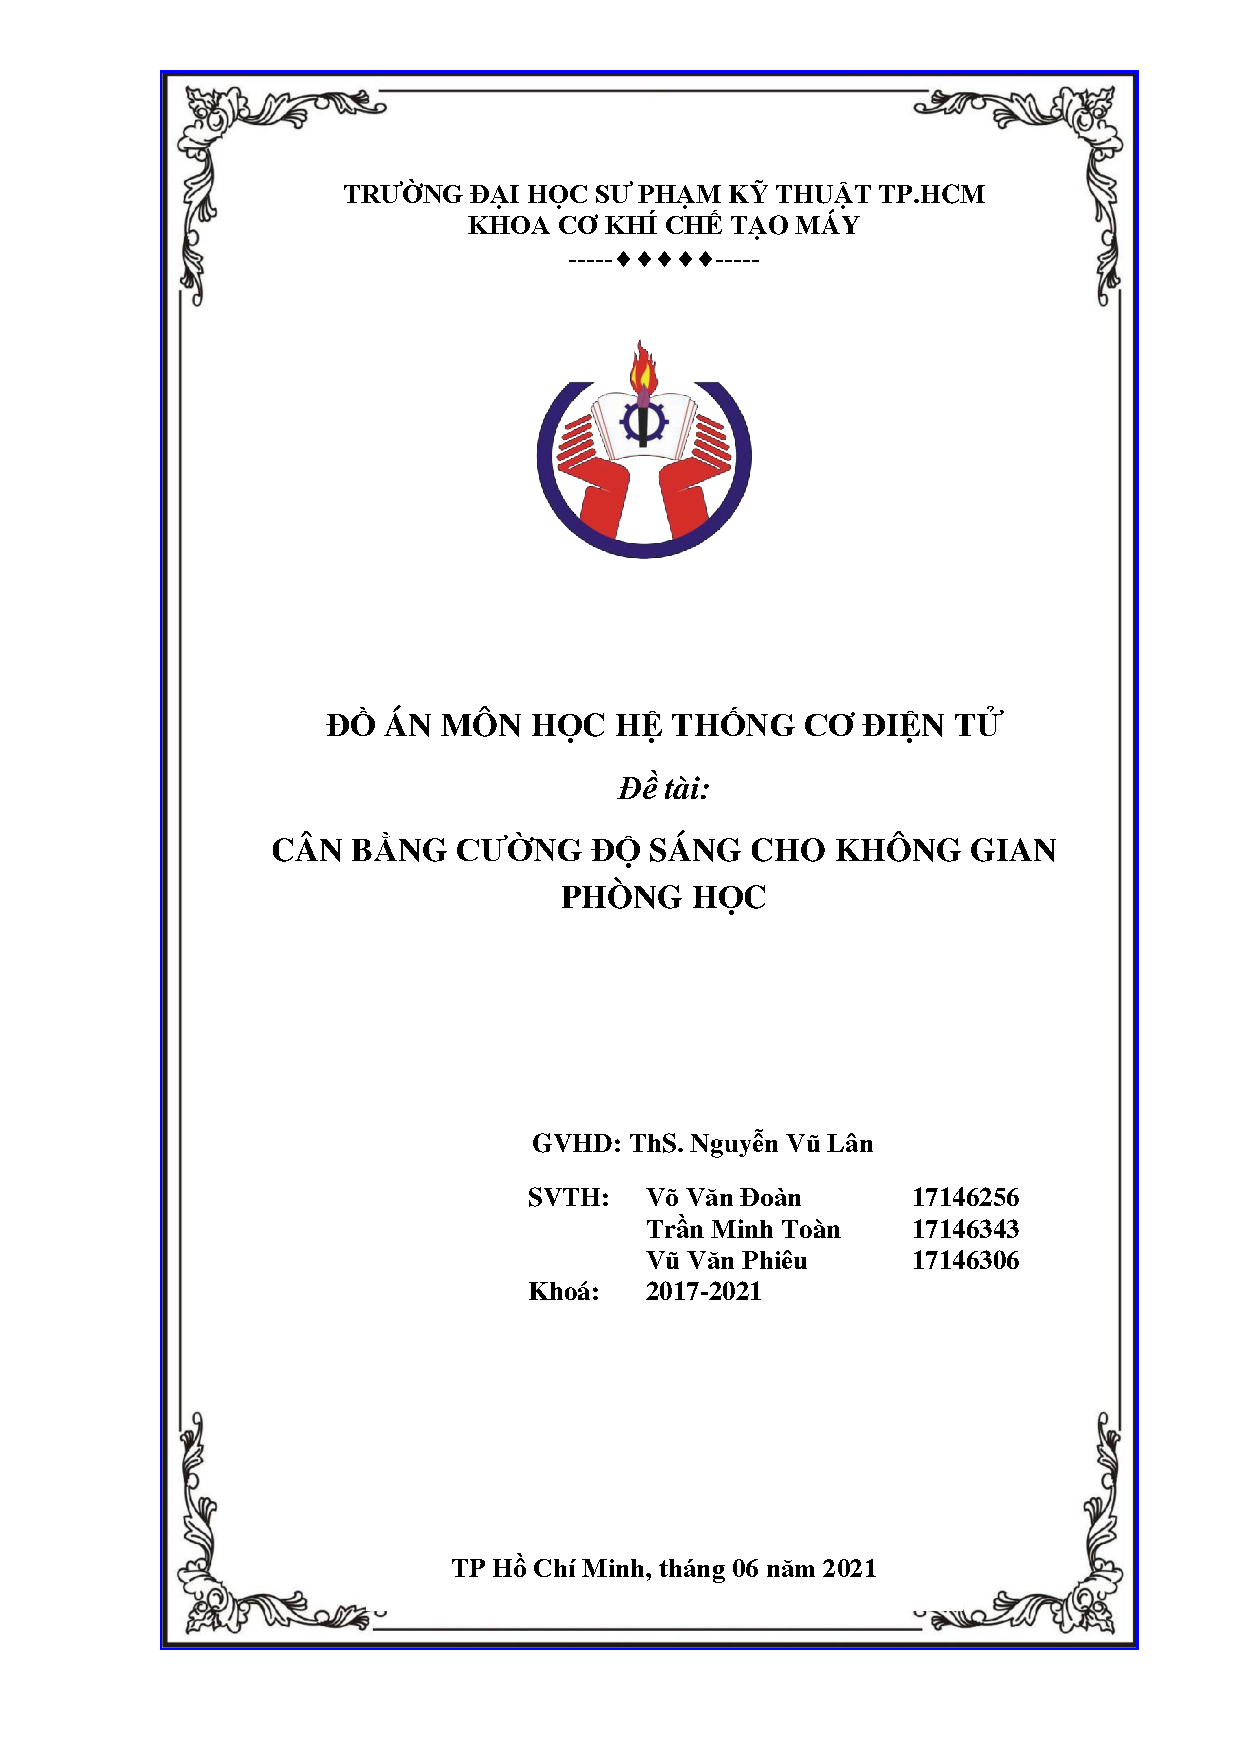
\includepdf[page=-]{Bia.pdf}
\setcounter{page}{1}
\begin{table}
\centering
\footnotesize
\begin{tabular}{p{0.5\linewidth} p{0.5\linewidth}}

\begin{center}
\makecell{TRƯỜNG ĐẠI HỌC SƯ PHẠM KỸ THUẬT \\ TP HCM}

KHOA CƠ KHÍ CHẾ TẠO MÁY
\end{center} & 
\begin{center}
CỘNG HOÀ XÃ HỘI CHỦ NGHĨA VIỆT NAM

\textit{Độc Lập - Tự Do - Hạnh Phúc}
\end{center} \\ 
\end{tabular} 
\end{table}
\begin{center}
\subsection*{NHIỆM VỤ ĐỒ ÁN MÔN HỌC HỆ THỐNG CƠ ĐIỆN TỬ}
\end{center}
\addcontentsline{toc}{section}{NHIỆM VỤ ĐỒ ÁN MÔN HỌC HỆ THỐNG CƠ ĐIỆN TỬ}

\textbf{Giảng viên hướng dẫn: } ThS Nguyễn Vũ Lân

\textbf{Sinh viên thực hiện: }
\begin{center}
\begin{tabular}{cc}
Võ Văn Đoàn & 17146256 \\ 

Trần Minh Toàn & 17146343 \\ 

Vũ Văn Phiêu & 17146306 \\ 
\end{tabular} 
\end{center}

\textbf{1. Tên đề tài: } Cân bằng cường độ sáng cho không gian phòng học.

\textbf{2. Các số liệu, tài liệu ban đầu: }

Kích thước mô hình phòng học: $ 1000 \times 600 \times 300 $ (Dài $\times$ rộng $\times$ cao).

\textbf{3. Nội dung chính của đồ án: }
\begin{itemize}
\item Thiết kế, thi công, lắp đặt mô hình phòng học.
\item Thi công, lắp đặt hệ thống động cơ, hệ thống đèn chiếu sáng.
\item Lắp đặt hệ thống cảm biến ánh sáng.
\item Viết chương trình điều khiển trên VĐK và phần mềm điều khiển trên PC.
\end{itemize}

\textbf{4. Các sản phẩm dự kiến: }
\begin{itemize}
\item Mô hình phòng học.
\item Hệ thống điều khiển.
\item Phần mềm điều khiển.
\end{itemize}

\textbf{5. Ngày giao đồ án: } 09/03/2021

\textbf{6. Ngày nộp đồ án: } 25/06/2021

\textbf{7. Ngôn ngữ trình bày: }
\begin{itemize}
\item Bản bảo cáo: Tiếng Việt.
\item Trình bày phản biện: Tiếng Việt.
\end{itemize}

\begin{center}
\begin{tabular}{w{c}{0.3\linewidth} w{c}{0.3\linewidth} w{c}{0.3\linewidth}}

\textbf{TRƯỞNG KHOA} & \textbf{TRƯỞNG BỘ MÔN} & \textbf{GVHD} \\ 

\textit{(Ký, ghi rõ họ tên)} & \textit{(Ký, ghi rõ họ tên)} & \textit{(Ký, ghi rõ họ tên)} \\ 

\end{tabular} 
\end{center}

\chapter*{LỜI CẢM ƠN}
\addcontentsline{toc}{section}{LỜI CẢM ƠN}
Tri thức chỉ khi được áp dụng vào thực tế thì việc chiếm lĩnh tri thức đó mới có giá trị. Điều này đặc biệt đúng trong các khối ngành Kỹ thuật, trong đó có ngành CNKT Cơ điện tử. Ở học kỳ trước, chúng em đã được kiểm tra, học hỏi, nghiên cứu thêm các kiến thức thi công một hệ thống cơ khí thực tế bằng đồ án Truyền động điều khiển. Kỳ này, chúng em tiếp tục được học hỏi, áp dụng các kiến thức đã được học, đồng thời kiểm tra năng lực của bản thân bằng cách thực hiện Đồ án môn học Hệ thống Cơ điện tử.

Lời đầu tiên, chúng em xin cảm ơn các quý thầy cô ở Khoa Cơ khí Chế tạo máy – Trường Đại học Sư Phạm Kỹ Thuật Thành phố Hồ Chí Minh, trong suốt những năm qua vẫn luôn tận tuỵ truyền đạt, giảng dạy vốn kiến thức, kinh nghiệm quý báu của mình cho các thế hệ sinh viên, trong đó có các sinh viên chuyên ngành CNKT Cơ điện tử như chúng em.

Để hoàn thành được đồ án này thì không thể thiếu một người giáo viên hướng dẫn trực tiếp tận tâm, giàu kinh nghiệm. Chúng em xin chân thành cảm ơn thầy giáo \textbf{Nguyễn Vũ Lân}, là giảng viên hướng dẫn của nhóm em. Nhờ sự giúp đỡ nhiệt tình, những đóng góp quan trọng và những lời phê bình sâu sắc của thầy, chúng em mới có thể hoàn thành tốt đồ án này. Em xin gửi đến thầy lời cảm ơn chân thành nhất. Kính chúc thầy luôn dồi dào sức khoẻ và công tác tốt.

Đề tài: \textbf{“Cân bằng cường độ sáng cho không gian phòng học”} được thực hiện vào học kỳ 2 năm học 2020 – 2021. Đề tài này ở cả trong nước và nước ngoài còn khá mới, bước đầu tìm tòi và nghiên cứu với kiến thức còn hạn chế và còn nhiều bỡ ngỡ, chúng em chắc chắn không thể tránh khỏi những thiếu sót. Để việc thực hiện Đồ án tốt nghiệp sau này cũng với đề tài này được thuận lợi, chúng em rất mong có được những ý kiến đóng góp của các quý Thầy cô trong Khoa Cơ khí – Chế tạo máy để đề tài được thực hiện đầy đủ và hiệu quả hơn. 
\begin{center}
\begin{tabular}{w{c}{0.5\linewidth} w{c}{0.5\linewidth}}
 & \textbf{Sinh viên thực hiện} \\ 
 & Võ Văn Đoàn \\ 
 & Trần Minh Toàn \\ 
 & Vũ Văn Phiêu \\  
\end{tabular} 
\end{center}


\tableofcontents

\chapter*{DANH MỤC TỪ VIẾT TẮT}
\addcontentsline{toc}{section}{DANH MỤC TỪ VIẾT TẮT}
\begin{center}
	\begin{tabular}{|c|c|c|}
	\hline 
	STT & Ký hiệu chữ viết tắt & Chữ viết đầy đủ \\ 
	\hline 
	1 & GUI & Graphical User Interface \\ 
	\hline 
	2 & VĐK & Vi điều khiển \\ 
	\hline 
	\end{tabular} 
\end{center}


\listoftables
\addcontentsline{toc}{section}{DANH SÁCH BẢNG}
\listoffigures
\addcontentsline{toc}{section}{DANH SÁCH HÌNH VẼ}

\chapter{GIỚI THIỆU}
\pagenumbering{arabic}
%\chapter{GIỚI THIỆU}

\section{Lý do chọn đề tài}

\begin{wrapfigure}{r}[0pt]{0.45\linewidth}
    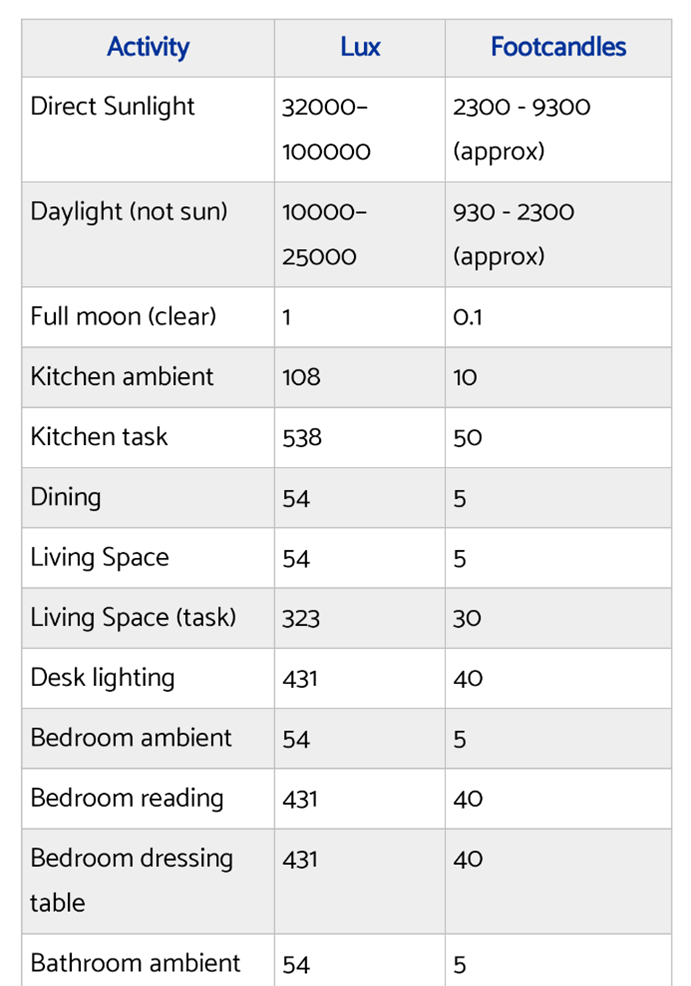
\includegraphics[scale=0.8]{Chapters/Chapter1/Images/Cuongdosangcanthiet}
    \caption{Bảng cường độ ánh sáng cần thiết cho các phòng}
    \label{fig:cuongdoanhsang}
\end{wrapfigure}

Trong hầu hết các hoạt động làm việc, sinh hoạt hằng ngày của con người, luôn cần một lượng ánh sáng nhất định. Tuỳ từng nơi sinh hoạt là phòng khách, phòng ăn (nhà ở) hay là phòng họp, nhà kho (công ty) mà chúng ta sẽ có mức cường độ ánh sáng cần thiết là khác nhau. Có thể thấy trong hình bên, trong nhà bếp, phòng ăn chúng ta chỉ cần 54 lux (đơn vị đo cường độ ánh sáng) còn trong khi đọc sách, chúng ta cần 431 lux. Hiện nay, gần như tất cả các phương án chiếu sáng đều đang sử dụng đèn cố định, tức là không thể thay đổi độ sáng lẫn góc chiếu, vị trí chiếu. Việc này dẫn tới hai nhược điểm sau đây:


Thứ nhất, vào ban ngày khi có ánh sáng tự nhiên, để tránh tình trạng hao phí điện năng thì chúng ta sẽ tắt đèn. Nhưng thường chỉ có những nơi gần cửa sổ, cửa ra vào mới được nhận lượng ánh sáng đầy đủ. Còn ở những nơi xa các nguồn sáng tự nhiên như góc phòng, giữa lớp sẽ có hiện tượng ánh sáng không đủ. Đối với các học sinh sinh viên khi học tập lâu dài trong điều kiện này sẽ dẫn tới các bệnh, tật về mắt.
\begin{center}
    \begin{figure}[ht]
    \begin{center}
     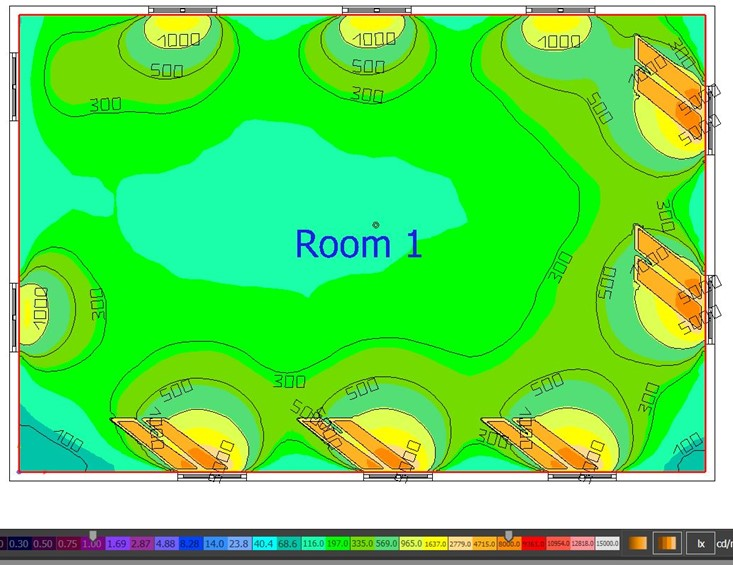
\includegraphics[scale=1]{Chapters/Chapter1/Images/Doroi}
    \end{center}
    \caption{Ảnh hưởng của ánh sáng tự nhiên tới cường độ ánh sáng trong phòng}
    \label{fig:doroi}
    \end{figure}
\end{center}

Thứ hai, thường hệ thống đèn chiếu trong phòng học dùng một vài công tắc để bật tắt toàn bộ đèn trong phòng. Nếu chúng ta bật đèn để khắc phục tình trạng trên thì lại dẫn đến một nhược điểm khác, đó là những nơi có ánh sáng tự nhiên sẽ dư thừa ánh sáng không cần thiết. Khi thiết kế hệ thống chiếu sáng, người thiết kế đã đảm bảo hệ thống đèn sẽ chiếu đủ ánh sáng cần thiết trong điều kiện ban đêm. Khi kết hợp với ánh sáng ban ngày thì sẽ bị dư thừa, gây hao phí điện nặng không cần thiết. Hiện tại, thế giới đang đối mặt với tình trạng nóng lên toàn cầu, việc cắt giảm lượng dư thừa này được áp dụng trên phạm vi rộng chắc chắn sẽ cải thiện một phần nhỏ hiện tượng này. Ngoài ra, việc cắt giảm lượng ánh sáng dư thừa sẽ giúp cho các nhà trường tiết kiệm một khoản tiền điện, điều này có lợi cho ngân sách nhà nước đối với các trường công lập và giảm bớt chi phí phải bỏ ra trong chiếu sáng cho các trường tư, tự chủ.

Do đó, nhóm đã chọn đề tài “ Cân bằng cường độ ánh sáng trong không gian phòng học” với mong muốn có thể cân bằng ánh sáng đều trên cả phòng học, giúp đảm bảo lượng ánh sáng cần thiết trong hoạt động học tập của học sinh, sinh viên và  góp phần tiết kiệm điện năng.

\section{Đối tượng nghiên cứu}
Đối tượng nghiên cứu của đề tài “ Cân bằng cường độ ánh sáng trong không gian phòng học” là: tập trung tìm hiểu, nghiên cứu các vấn đề liên quan, thiết kế và thi công mô hình điều khiển, đưa ra các giải thuật để cân bằng ánh sáng cho không gian trong phòng học.

\section{Mục tiêu nghiên cứu}
\begin{itemize}
\item Đưa ra được các giải thuật cân bằng cường độ ánh sáng trong phòng học.
\item Thực hiện được mô hình phòng học được cân bằng cường độ ánh sáng.
\end{itemize}

\section{Giới hạn đề tài}
Đề tài thực hiện nghiên cứu, thiết kế và thi công mô hình thử nghiệm ở mức độ:
\begin{itemize}
\item Điều khiển cường độ ánh sáng thông qua màn hình máy tính, nút nhấn.
\item Cân bằng bằng cách điều khiển cường độ sáng của đèn hoặc tịnh tiến đèn để đạt được cường độ sáng cần thiết ở mọi điểm trong phòng.
\end{itemize}

\section{Phương pháp nghiên cứu}
Các vấn đề cần nghiên cứu trong đề tài:
\begin{itemize}
\item Phần cứng: Lắp ráp khung mô hình, bộ phận trượt cho dàn đèn, thi công đi dây cho mạch điện, driver điều khiển động cơ step, cảm biến và đèn công suất.
\item Phần mềm: Phần mềm giao tiếp với VĐK từ máy tính bằng giao tiếp UART, chương trình điều khiển hệ thống của VĐK.
\end{itemize}
Phương pháp nghiên cứu:
\begin{itemize}
\item Tìm hiểu tài liệu: tìm hiểu các tài liệu về cường độ sáng, thiết kế chiếu sáng, các phương pháp điều khiển.
\item Tự nghiên cứu: thông qua các tài liệu và các phương tiện thông tin, nhóm tự xây dựng giải thuật, cách xây dựng chương trình.
\item Phương pháp thực nghiệm, thử và thử sai: thực nghiệm điều khiển cân bằng cường độ sáng, qua đó rút ra được kinh nghiệm.
\end{itemize}

\section{Phương pháp thiết kế chung}
\begin{itemize}
\item Sản phẩm: Lập trình điều khiển để cân bằng cường độ ánh sáng trong phòng.
\item Năng suất: Mô hình có thể điều khiển cân bằng ánh sáng với thời gian ngắn và độ chính xác cao.
\item Các thiết kế cơ khí được thiết kế phù hợp với phòng học thực tế.
\end{itemize}







\chapter{TỔNG QUAN}
\section{Các nghiên cứu có liên quan ngoài nước}
Hiện nay tại các nước phát triển thì chiếu sáng nhân tạo là một vấn đề được rất nhiều công ty, tổ chức quan tâm và nghiên cứu. Chiếu sáng nhân tạo phục vụ các nhu cầu khác nhau: như trồng cây trong nhà kính, chiếu sáng các văn phòng, các phòng học… Tuy phục vụ các nhu cầu khác nhau nhưng điểm chung giữa các nghiên cứu ấy đều tập trung điều chỉnh cường độ ánh sáng và độ rọi lên bề mặt cần chiếu sáng.

Tại Farmertyler, một công ty tư vấn nông nghiệp chuyên về nông nghiệp đô thị, thủy canh, canh tác thẳng đứng và sản xuất nhà kính, ánh sáng được điều chỉnh và lựa chọn màu sắc phù hợp để kích thích và làm cho cây trồng phát triển và sinh trưởng nhanh. (Hình~\ref{fig:nhakinhtrongrau})
\begin{center}
    \begin{figure}[!htp]
    \begin{center}
     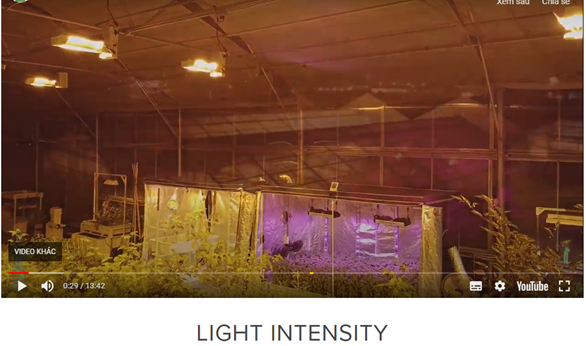
\includegraphics[scale=0.9]{Chapters/Chapter2/ImagesChapter2/Nhakinhtrongrau}
    \end{center}
    \caption{Cân bằng ánh sáng trong nhà kính trồng rau}
    \label{fig:nhakinhtrongrau}
    \end{figure}
\end{center}

Theo như bài nghiên cứu của tác giả: Sanaz Sanami thuộc Payame Noor University với bài nghiên cứu: “The Impact of Indoor Lighting on Students’ Learning Performance in Learning”. Bài nghiên cứu chỉ ra cho chúng ta thấy tác động của chiếu sáng trong phòng ảnh hưởng đến hiệu quả học tập của học sinh.

Hay như một bài nghiên cứu của Đại học Monash về ánh sáng nhân tạo tới nhịp sinh học thì PGS Cain cho biết: “Sự cân bằng âm và dương cũng là sự cân bằng giữa ánh sáng và bóng tối. Và sự cân bằng này rất quan trọng đối với việc điều tiết hệ thống sinh lý học của chúng ta. Ánh sáng nhân tạo phá vỡ nhịp hoạt động này, làm rối loạn giấc ngủ, ảnh hưởng đến sức khỏe và là nguyên nhân dẫn đến nhiều bệnh mãn tính hơn”.

\section{Các nghiên cứu có liên quan trong nước}
Hiện nay trong nước thì vấn đề về chiếu sáng trong phòng cũng chưa được quan tâm nhiều. Ở các phòng học và các công xưởng thì vấn đề chiếu sáng chỉ dừng ở mức độ chiếu đủ độ sáng. (Hình~\ref{fig:nhakho})
\begin{center}
    \begin{figure}[!htp]
    \begin{center}
     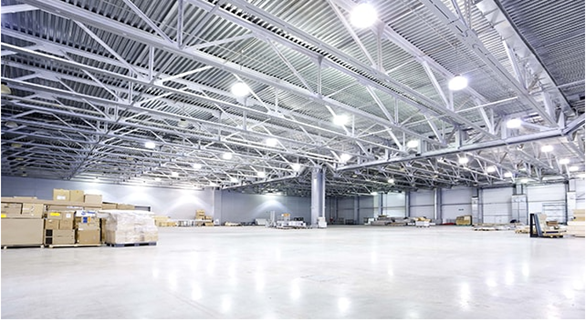
\includegraphics[scale=0.9]{Chapters/Chapter2/ImagesChapter2/Nhakho}
    \end{center}
    \caption{Chiếu sáng trong nhà kho}
    \label{fig:nhakho}
    \end{figure}
\end{center}

Ở các phòng công nghiệp thì ánh sáng được lắp và phân bố đều nhưng chỉ đảm bảo độ sáng chứ chưa có chuyên sâu về mức độ đảm bảo sức khỏe.

Công ty FSIVN, chuyên cung cấp các giải pháp thiết kế chiếu sáng trường học. Hình dưới là giải pháp của công ty cho một phòng học với ánh sáng trải đều, đèn điện có máng che đèn điện lắp so le và không có loáng của quạt. (Hình~\ref{fig:lophoc})

Từ hình ảnh trên chúng ta cũng thấy được ưu điểm của phương pháp này là ánh sáng của căn phòng luôn đạt được độ sáng chênh lệch và dao động từ 300-500 lux. Nhưng nhược điểm của nó là có thể thấy vào những ngày thời tiết khác nhau cường độ ánh sáng bên ngoài tác động vào thì ánh sáng trong phòng sẽ khác, có nơi cường độ ánh sáng cao hơn mức cho phép và cũng có những nơi không đạt được độ sáng cần thiết.
\begin{center}
    \begin{figure}[!htp]
    \begin{center}
     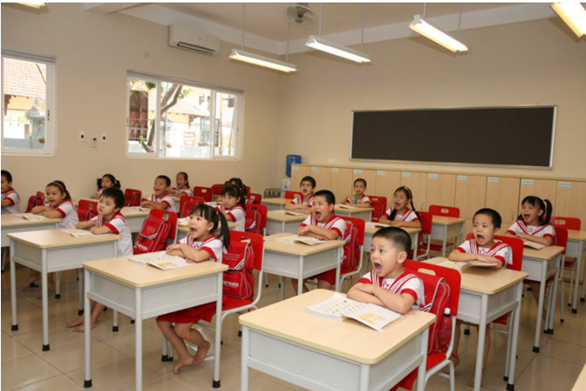
\includegraphics[scale=0.9]{Chapters/Chapter2/ImagesChapter2/Lophoc}
    \end{center}
    \caption{Chiếu sáng trong lớp học}
    \label{fig:lophoc}
    \end{figure}
\end{center}

\section{Hướng nghiên cứu và phát triển}
Từ các bài nghiên cứu ở ngoài nước và trong nước thì chúng ta có thể thấy tầm quan trọng của ánh sáng nhân tạo hiện nay rất quan trọng. Tác động tích cực và tiêu cực của nó đối với con người và sinh vật rất lớn.

Nhận thấy tính quan trọng và cấp thiết của vấn đề. Nhóm chúng em lựa chọn nghiên cứu “Hệ thống cân bằng ánh sáng trong phòng kín” với mục đích là đề ra là tạo ra hệ thống cung cấp đủ ánh sáng trong phòng, cung cấp ánh sáng với độ rọi phù hợp. Hệ thống được xây dựng với định hướng nghiên cứu:
\begin{itemize}
\item Cung cấp ánh sáng trải đều trên diện tích chiếu sáng.
\item Hệ thống tự điều chỉnh được bố cục đèn.
\item Hệ thống tự đo và điều chỉnh cường độ ánh sáng khi có tác động ánh sáng khác từ bên ngoài.
\item Báo cáo liên tục cho người dùng độ sáng của đèn.
\item Đưa ra khuyến nghị khi ánh sáng trong phòng thay đổi. 
\end{itemize}



\chapter{PHÂN TÍCH ĐỀ TÀI VÀ PHƯƠNG ÁN THIẾT KẾ}
\section{Thông số thiết kế}

\begin{center}
    \begin{figure}[ht]
    \begin{center}
     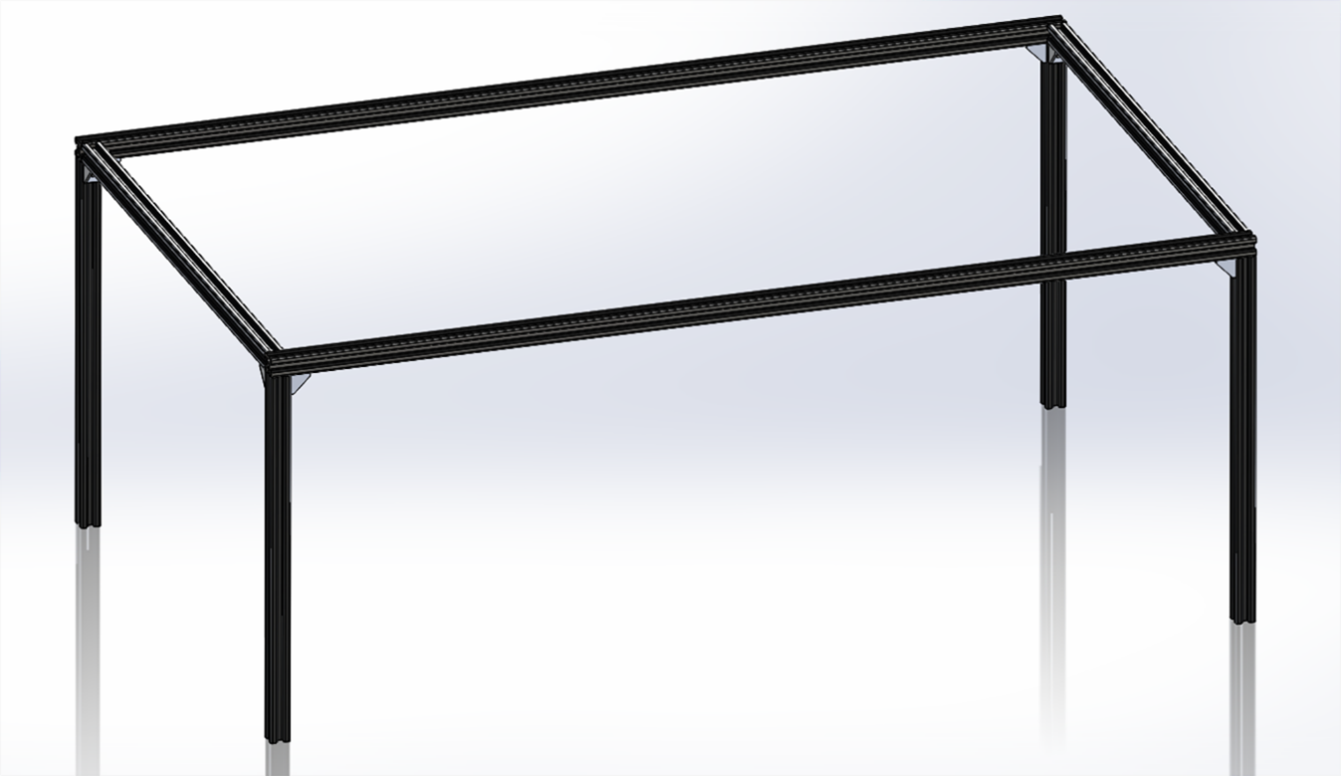
\includegraphics[scale=1]{Chapters/Chapter3/Images/Khungnhomdinhhinh}
    \end{center}
    \caption{Khung nhôm định hình}
    \label{fig:khungnhom}
    \end{figure}
\end{center}

Kích thước khung: 1000 x 600 x 400 mm (dài x rộng x cao).

\section{Phương hướng và giải pháp thực hiện}
Để thiết kế được hệ thống đèn có thể điều chỉnh để nhầm ứng cường độ sáng tại các điểm, ta cần giải quyết được các vấn đề:
\begin{itemize}
\item Tịnh tiến được các dàn đèn
\item Điều khiển dễ dàng, chính xác.
\item Không gây tiếng ồn đáng kể.
\end{itemize}

Dựa theo đó, ta có các phương án sau:

\subsection{Phương án 1}
Ta tịnh tiến các dàn đèn bằng chuyển động trượt, dùng các con lăn nhôm V-slot trượt trên nhôm (Hình~\ref{fig:phuongan1}).
\begin{center}
    \begin{figure}[ht]
    \begin{center}
     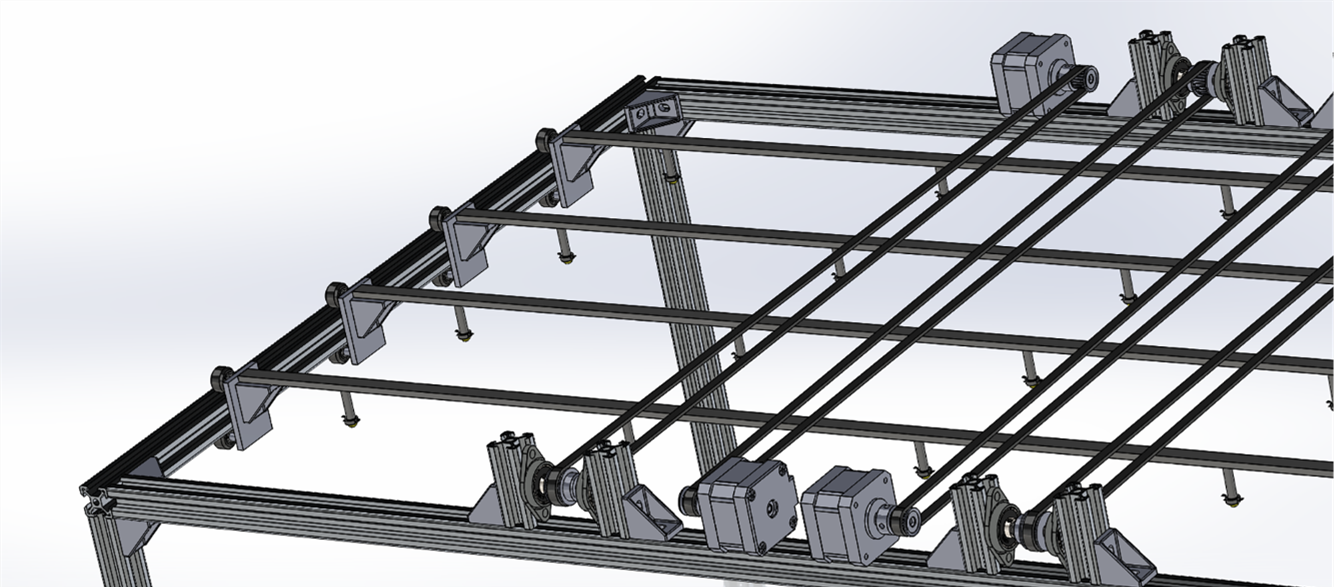
\includegraphics[scale=1]{Chapters/Chapter3/Images/Phuongan1}
    \end{center}
    \caption{Phương án 1}
    \label{fig:phuongan1}
    \end{figure}
\end{center}

\subsection{Phương án 2}
Ta tịnh tiến các dàn đèn bằng chuyển động trượt, dùng 2 con trượt vuông chuyển động trên ti trượt (Hình~\ref{fig:phuongan2}). 
\begin{center}
    \begin{figure}[htp]
    \begin{center}
     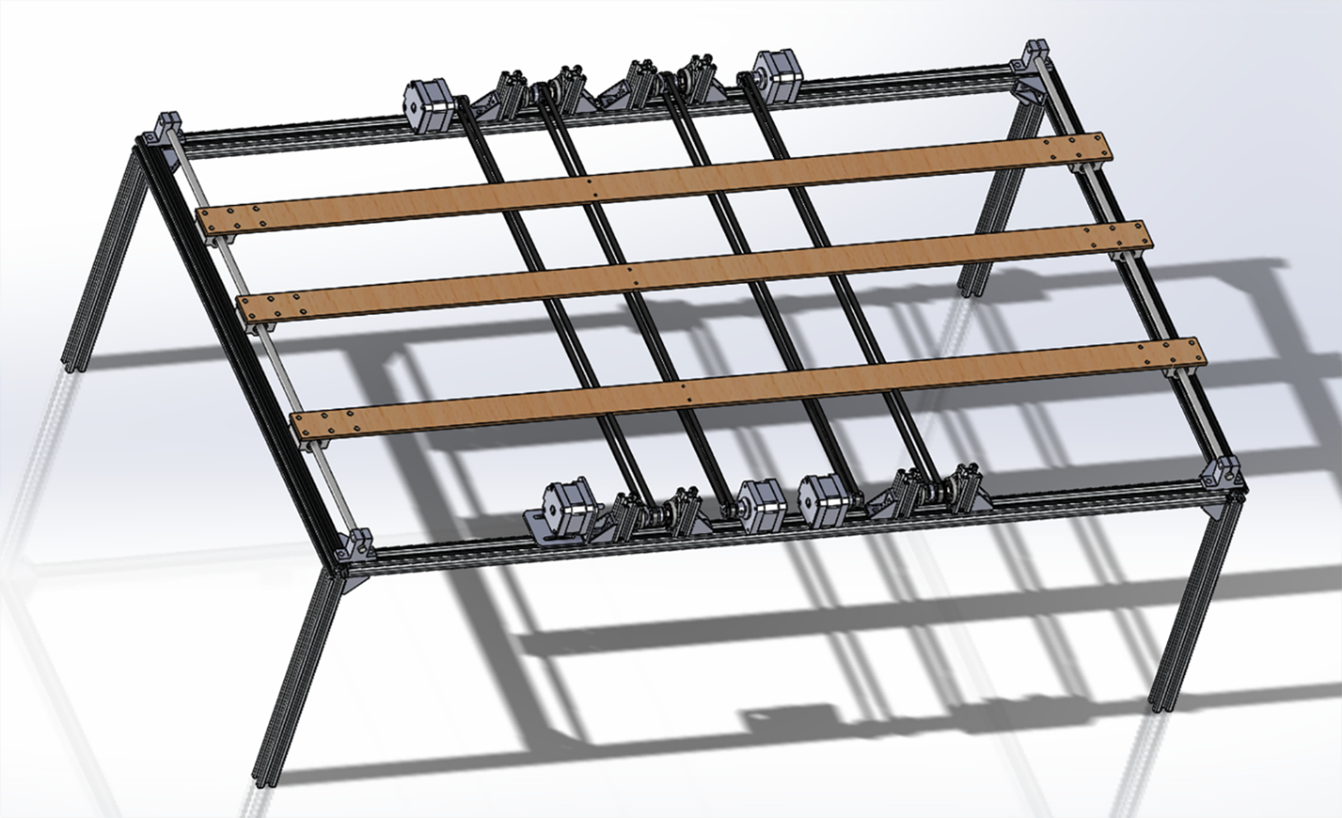
\includegraphics[scale=1]{Chapters/Chapter3/Images/Phuongan2}
    \end{center}
    \caption{Phương án 2}
    \label{fig:phuongan2}
    \end{figure}
\end{center}

\subsection{Phương án 3}
Ta tịnh tiến các dàn đèn bằng chuyển động trượt, dùng 2 con trượt vuông chuyển động trên ti trượt (Hình~\ref{fig:phuongan3}). 
\begin{center}
    \begin{figure}[htp]
    \begin{center}
     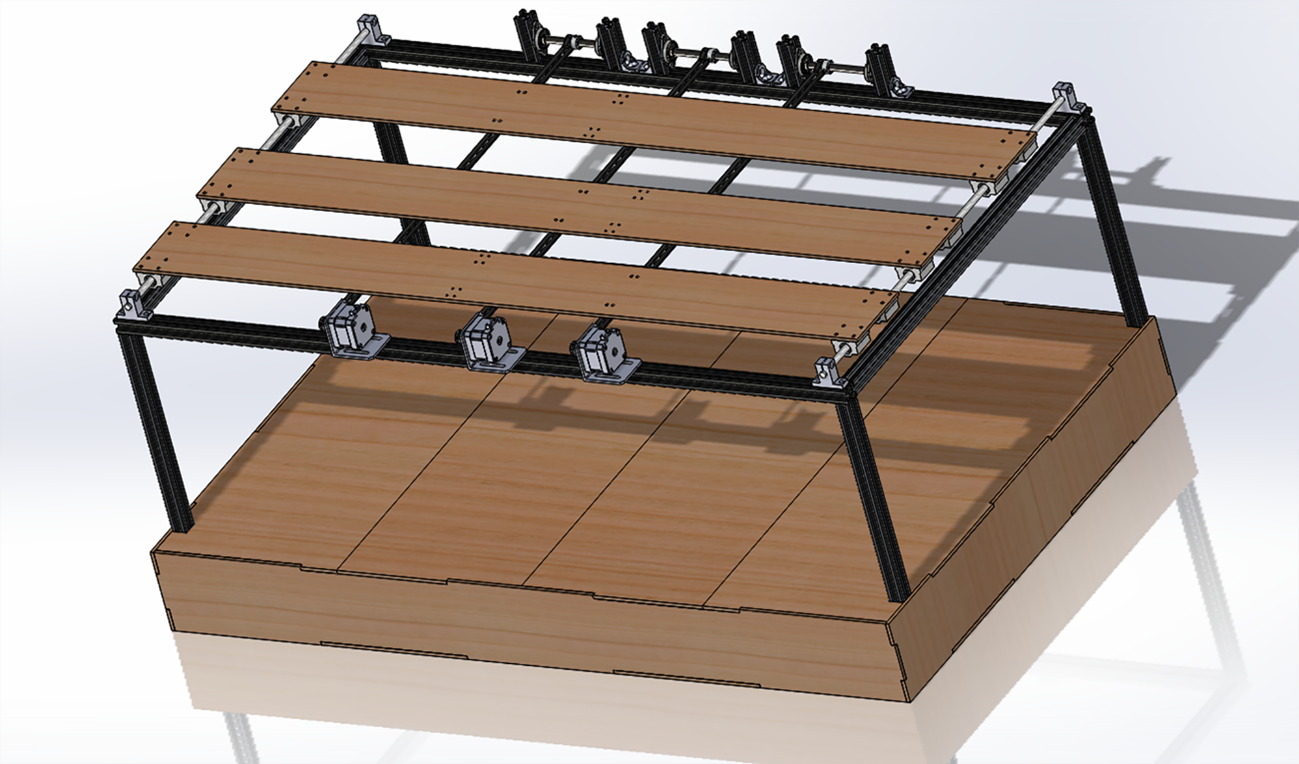
\includegraphics[scale=1]{Chapters/Chapter3/Images/Phuongan3}
    \end{center}
    \caption{Phương án 3}
    \label{fig:phuongan3}
    \end{figure}
\end{center}

\subsection{Lựa chọn phương án tối ưu:}

\begin{table}[H]
\centering
\begin{tabular}{|c|c|c|c|}
\hline 
Đặc điểm & Phương án 1 & Phương án 2 & Phương án 3 \\ 
\hline 
Ổn định & + & - & + \\ 
\hline 
Chi phí & - & + & + \\ 
\hline 
Chính xác & - & - & + \\ 
\hline 
Cơ cấu đơn giản & - & + & + \\ 
\hline 
Khả năng lắp ráp, thay thế & + & + & + \\ 
\hline 
Không gian hoạt động & + & + & - \\ 
\hline 
\textbf{Tổng} & 3+ & 4+ & 5+ \\ 
\hline 
\end{tabular} 
\caption{So sánh các phương án thiết kế cơ cấu truyền động}
\label{tab:sosanhcokhi}
\end{table}

Sau khi so sánh ưu nhược điểm của từng phương án, nhóm quyết định lựa chọn phương án 3. (Bảng \ref{tab:sosanhcokhi})

\section{Chọn động cơ}
\begin{table}[H]
\centering
\begin{tabular}{|c|p{5.5cm}|p{5.5cm}|}
\hline
 & Động cơ STEP & Động cơ DC Servo \\
\hline 
Ưu điểm & 
- Tạo ra chuyển động gia tăng, giảm chi phí và độ phức tạp của bộ mã hóa.

- Số cực cao nên có thể tạo ra mô-men xoắn rất cao ở tốc độ 0.

- Kích thước nhỏ gọn, tiết kiệm chi phí.
& 
- Là hệ thống hồi tiếp vòng kín chính vì vậy động cơ servo DC rất dễ điều khiển, dễ sử dụng.

- Mô-men xoắn khởi động lớn.

- Có thể được sử dụng trong các ứng dụng công nghiệp và dân dụng nói chung nhạy cảm với chi phí. \\ 
\hline 
Nhược điểm & 
- Tốc độ bị giới hạn, chạy tốt nhất ở 1200 vòng/phút hoặc thấp hơn.

- Mặc dù tạo mô-men xoắn cao ở tốc độ 0, nhưng mô-men xoắn sẽ rơi khi tốc độ tăng.
 & 
- Vì cấu tạo có bộ phận chổi than nên điểm hạn chế lớn nhất của loại động cơ này chính là dễ gây ra tiếng ồn, nhiệt độ cao.

- Quán tính cao khi giảm tốc độ.

- Bảo trì bất tiện (thay thế chổi than). \\ 
\hline 
\end{tabular} 
\caption{Bảng so sánh động cơ Step và động cơ DC Servo}
\label{tab:sosanhdongco}
\end{table}

Trong kỹ thuật không có giải pháp nào hoàn hảo, mà chỉ được coi là giải pháp tốt nhất, đặc biệt đối với động cơ SERVO và động cơ STEP. Cả hai đều được sử dụng rộng rãi trong ngành công nghiệp. Khi được áp dụng đúng cách, hai động cơ này đều có thể mang lại hiệu quả làm việc đáng mong đợi cho cả hệ thống máy. Để đi tới quyết định lựa chọn loại động cơ nào phù hợp thì phụ thuộc vào rất nhiều yếu tố, nhưng quan trọng nhất là tốc độ, gia tốc và giá cả.


Vì trong đề tài này, nhóm thực hiện mô hình với kích thước nhỏ, với mục đích điều khiển dễ dàng, chính xác và không gây tiếng ồn với chi phí thấp, dễ thay thế, bảo trì nên qua việc phân tích những ưu điểm và nhược điểm của hai loại động cơ này (Bảng~\ref{tab:sosanhdongco}), ta thấy động cơ STEP sẽ phù hợp với mô hình hơn.

\textbf{Động cơ bước NEMA17:} (Hình~\ref{fig:nema17})
\begin{center}
    \begin{figure}[htp]
    \begin{center}
     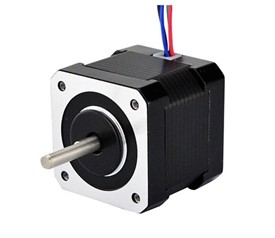
\includegraphics[scale=1]{Chapters/Chapter3/Images/NEMA17}
    \end{center}
    \caption{Động cơ bước NEMA17}
    \label{fig:nema17}
    \end{figure}
\end{center}
\begin{table}[H]
\centering
\begin{tabular}{|p{0.12\linewidth}|p{0.12\linewidth}|p{0.12\linewidth}|p{0.12\linewidth}|p{0.12\linewidth}|p{0.12\linewidth}|p{0.12\linewidth}|p{0.12\linewidth}|}
\hline 
Động cơ bước & Kích thước motor ($mm$) & Bước góc ($^{\circ}$) & Cường độ dòng điện ($A$) & Điện trở pha ($\Omega$) & Moment xoắn ($Nmm$) & Moment quán tính ($g.cm^2$) & Trọng lượng ($g$) \\
\hline 
NEMA 17 & $42x42$ & 1.8 & 1.7 & 5.75 & 280 & 100 & 300 \\
\hline 
\end{tabular} 
\caption{Bảng thông số kỹ thuật của động cơ NEMA17}
\label{tab:NEMA17}
\end{table}

\section{Lựa chọn các chi tiết cho mô hình}

\textbf{Nhôm định hình:} nhóm đã sử dụng nhôm định hình 20 x 20 để làm khung. (Hình~\ref{fig:nhomdinhhinh})

Ưu điểm:
\begin{itemize}
\item Có kết cấu vững chắc, bền vững với thời gian.
\item Không bị cong vênh, không bị oxi hóa, không biến đổi do nhiệt.
\item Ưu điểm vượt trội về khối lượng cũng như không bị mối mọt như gỗ.
\item Được sơn tĩnh điện, không bị bong sơn, tính thẩm mĩ cao.
\end{itemize}
\begin{center}
    \begin{figure}[htp]
    \begin{center}
     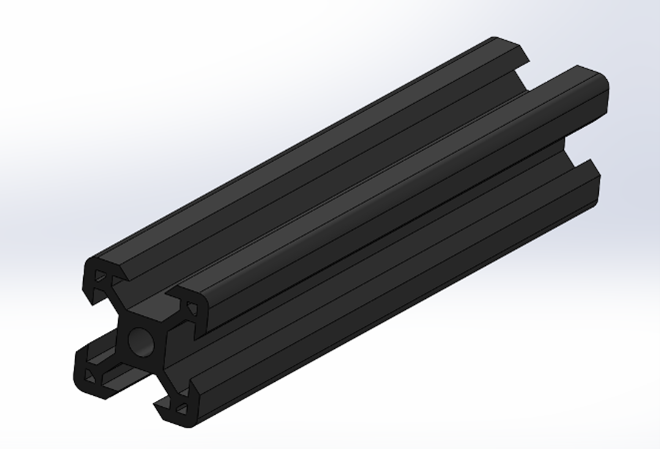
\includegraphics[scale=1]{Chapters/Chapter3/Images/Nhomdinhhinh}
    \end{center}
    \caption{Nhôm định hình 20x20}
    \label{fig:nhomdinhhinh}
    \end{figure}
\end{center}

\textbf{Ke góc vuông:} Ke sử dụng để cố định và gá các thanh nhôm tạo khung. (Hình~\ref{fig:kegocvuong})
\begin{center}
    \begin{figure}[htp]
    \begin{center}
     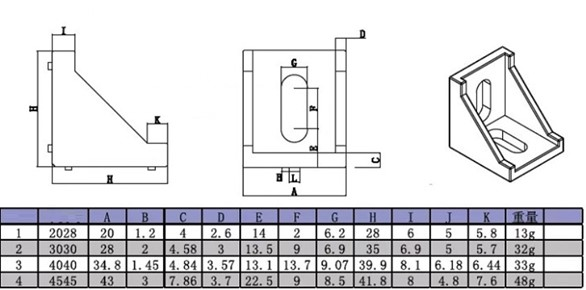
\includegraphics[scale=1]{Chapters/Chapter3/Images/Kegocvuong}
    \end{center}
    \caption{Ke góc vuông}
    \label{fig:kegocvuong}
    \end{figure}
\end{center}

\textbf{Gối đỡ trục:} Gối đỡ thanh trượt tròn 8mm dùng đỡ 2 đầu cho các thanh trượt tròn. (Hình~\ref{fig:goidotruc})
\begin{center}
    \begin{figure}[htp]
    \begin{center}
     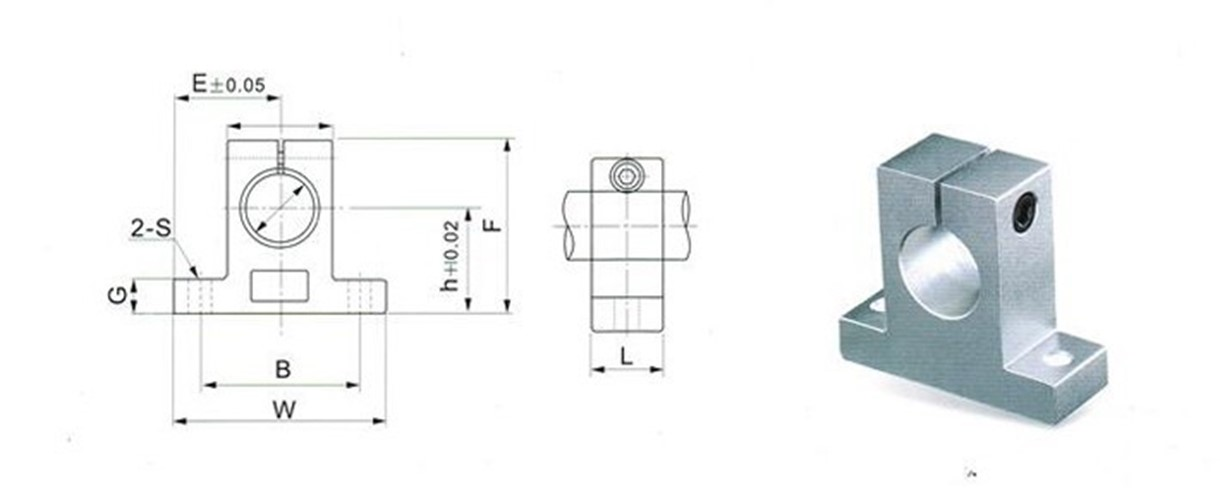
\includegraphics[scale=1]{Chapters/Chapter3/Images/Goidotruc}
    \end{center}
    \caption{Gối đỡ trục}
    \label{fig:goidotruc}
    \end{figure}
\end{center}
\begin{center}
    \begin{figure}[htp]
    \begin{center}
     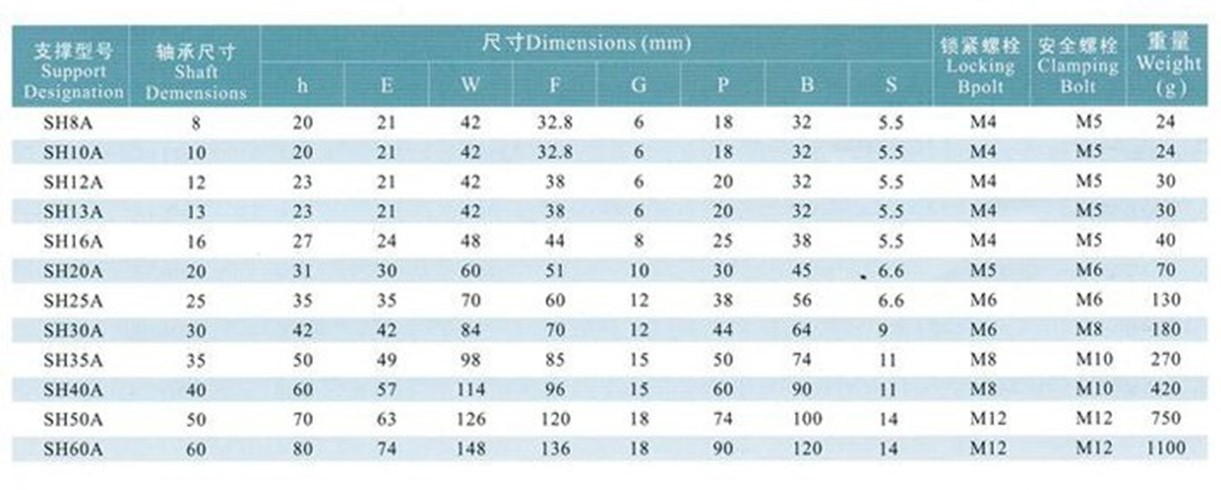
\includegraphics[scale=1]{Chapters/Chapter3/Images/Kichthuocgoidotruc}
    \end{center}
    \caption{Bảng kích thước gối đỡ trục}
    \label{fig:kichthuocgoidotruc}
    \end{figure}
\end{center}

\textbf{Con trượt vuông:} cho phép các chi tiết máy móc chuyển động tinh tiến chính xác, mượt mà, nhẹ nhàng, êm ái, ít lực ma sát nhất. (Hình~\ref{fig:contruotvuong})
\begin{center}
    \begin{figure}[htp]
    \begin{center}
     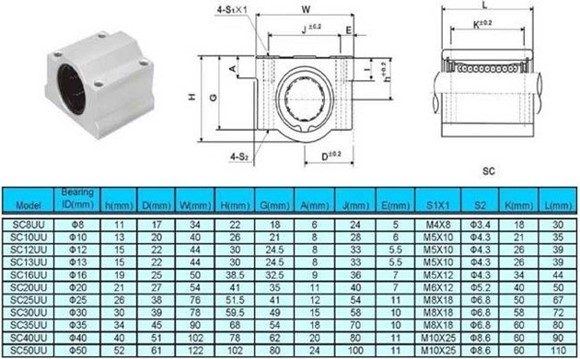
\includegraphics[scale=1]{Chapters/Chapter3/Images/Contruotvuong}
    \end{center}
    \caption{Con trượt vuông}
    \label{fig:contruotvuong}
    \end{figure}
\end{center}

\textbf{Gối đỡ vòng bi ngang:} (Hình~\ref{fig:goidovongbingang})

\begin{center}
    \begin{figure}[htp]
    \begin{center}
     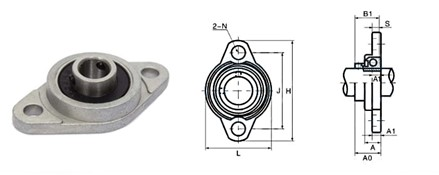
\includegraphics[scale=1]{Chapters/Chapter3/Images/Goidovongbingang}
    \end{center}
    \caption{Gối đỡ vòng bi ngang}
    \label{fig:goidovongbingang}
    \end{figure}
\end{center}

\textbf{Puly:} Pully có lỗ 5mm tương thích với đa số các động cơ bước, đặc biệt loại động cơ bước NEMA17. (Hình~\ref{fig:puly})
\begin{center}
    \begin{figure}[htp]
    \begin{center}
     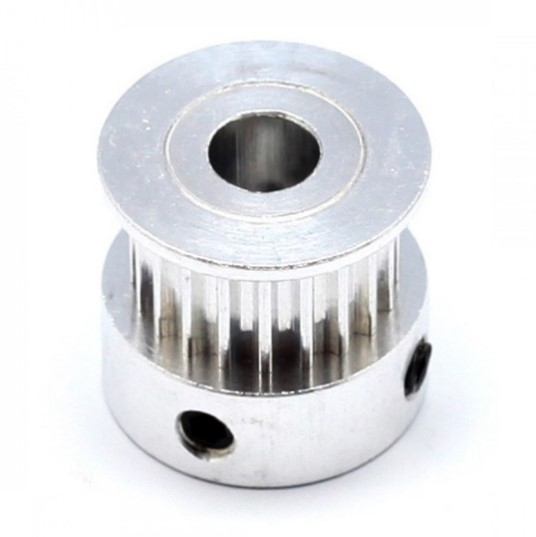
\includegraphics[scale=0.7]{Chapters/Chapter3/Images/Puly}
    \end{center}
    \caption{Puly trục 5mm 20 răng}
    \label{fig:puly}
    \end{figure}
\end{center}

\textbf{Dây đai GT2:} sử dụng profin bo tròn, bước răng 2mm đảm bảo các răng của đai khít vừa vặn và chính xác. (Hình~\ref{fig:daiGT2})
\begin{center}
    \begin{figure}[htp]
    \begin{center}
     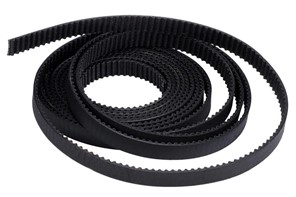
\includegraphics[scale=0.7]{Chapters/Chapter3/Images/DaiGT2}
    \end{center}
    \caption{Dây đai GT2}
    \label{fig:daiGT2}
    \end{figure}
\end{center}
\clearpage
\section{Tính toán lựa chọn đèn}
Vấn đề chiếu sáng trong văn phòng, trong các phòng kín luôn là vấn đề được nghiên cứu và phát triển. Mục đích chiếu sáng tạo ra môi trường ánh sáng tốt, tiện nghi, làm cho người sử dụng cảm thấy dễ chịu. Ngoài ra ở các giảng đường, thư viện hay các văn phòng kín , việc chiếu sáng giúp cho người học hay người làm cảm thấy làm việc học tập có hiệu quả hơn.

Yêu cầu của đèn khi thiết kế cần đảm bảo:
\begin{itemize}
\item Đảm bảo được độ rọi để phục vụ cho công việc, việc học tập.
\item Đảm bảo tiện nghi, không gây lóa mắt.
\item Màu sắc và nhiệt độ trong phòng phù hợp.
\item Vấn đề thẩm mỹ và tiết kiệm năng lượng.	
\end{itemize}

\subsection{Chọn độ rọi}
Độ rọi của đèn thể hiện được bề mặt làm việc, nơi đó còn gọi là “bề mặt hữu ích” với mô hình nhóm lựa chọn có độ cao là 300mm so với mặt sàn.

 Độ rọi này phụ thuộc vào góc chiếu của đèn, của chóa đèn….ở cấp độ mô hình thì nhóm mong muốn là giữa các phần giao thoa của đèn thì cường độ ánh sáng được đảm bảo với cường độ ánh sáng mong muốn.
 
 Hình \ref{fig:doroi} thể hiện ảnh hưởng của ánh sáng tự nhiên vào căn phòng, có thể thấy ở các vùng gần cửa sổ thì có cường độ ánh sáng cao nhưng ở nơi xa cửa sổ (trung tâm phòng học) có cường độ thấp hơn.

\subsection{Chọn loại đèn}
Việc lựa chọn đèn thích hợp nhất trong các loại đèn được nhóm triển khai theo các tiêu chuẩn sau đây:
\begin{itemize}
\item Góc chiếu của đèn đảm bảo được các vùng sáng giao thoa nhau.
\item Đèn có cường độ ánh sáng có thể điều chỉnh phù hợp.
\item Tuổi thọ của đèn.
\item Hiệu quả ánh sáng của đèn.
\item Chi phí.
\end{itemize}

\begin{center}
    \begin{figure}[ht]
    \begin{center}
     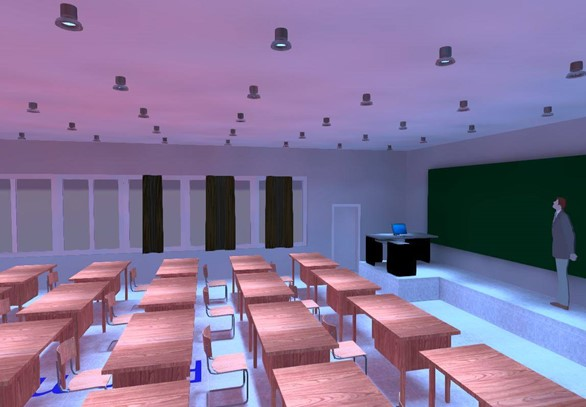
\includegraphics[scale=1]{Chapters/Chapter3/Images/Phonghocmophong}
    \end{center}
    \caption{Mô phỏng bố trí đèn chiếu trong phòng học sử dụng phần mềm DIALux}
    \label{fig:phonghocmophong}
    \end{figure}
\end{center}

\subsection{Chọn phương án chiếu sáng và bộ đèn}
Trong cuộc sống chúng ta thường gặp những cách chiếu sáng trực tiếp và bán trực tiếp. Kiểu chiếu sáng phụ thuộc vào các yếu tố ngoại quan như ánh sáng môi trường, thời tiết, khí hậu, tính phản xạ,…

Đối với loại đèn khác nhau, thì nhà sản xuất đã cung cấp catalog cho phép chọn kiểu bộ đèn, cấp xác định và nếu có thể người sản xuất đảm bảo có đủ các loại công suất khác nhau.

\subsection{Bố trí các đèn}
Không gian của nhóm thực hiện là không gian hình chữ nhật nên nhóm lựa chọn phương án bố trí đèn theo từng dàn cách đều nhau.

Bằng cách tính tổng quan thông số của đèn thì ta tính được số đèn tương ứng để chiếu sáng. Vì thế số đèn chọn là nhỏ nhất nhưng bố trí đều đặn sao cho khi sử dụng thì đèn sẽ đồng đều và độ rọi sẽ tốt nhất.

\subsection{Thực nghiệm và chọn loại đèn phù hợp}
Sau khi tìm hiểu các yêu cầu mà bóng đèn cần có thì nhóm đã tiến hành mô phỏng tính toán để chọn ra các loại đèn tối ưu nhất đáp ứng các nhu cầu đề ra và tiến hành lắp ráp thực tế. Các loại đèn được nhóm lựa chọn: đèn công suất siêu sáng 3W, 5W, 10W.


\textbf{Đèn LED công suất 10W:} (Hình~\ref{fig:10W})

Đèn siêu sáng 10W cung cấp ánh sáng trắng với cường độ cao có thể thay đổi được, trong khi thực tiễn thì mặc dù đáp ứng được độ sáng cho mô hình nhưng vẫn còn tồn tại rất nhiều nhược điểm như:

\begin{itemize}
\item Bóng tỏa một lượng nhiệt rất lớn.
\item Công suất tiêu thụ lớn.
\item Giá thành của bóng cao.
\item Việc điều khiển cường độ ánh sáng ở chế độ auto thì gặp nhiều cản trở do góc chiếu của đèn khá rộng.
\end{itemize}
\begin{center}
    \begin{figure}[ht]
    \begin{center}
     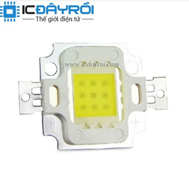
\includegraphics[scale=1]{Chapters/Chapter3/Images/Led10W}
    \end{center}
    \caption{Đèn LED công suất 10W}
    \label{fig:10W}
    \end{figure}
\end{center}

\textbf{Đèn LED công suất 5W:} (Hình~\ref{fig:5W})

Led 5W cung cấp ánh sáng trắng cho toàn bộ căn phòng, thỏa mãn các điều kiện cần của mô hình nhưng vẫn còn tồn tại là giá thành cao, và khi không có các yếu tố bên ngoài thì ánh sáng của led khi hoạt động ở trạng thái 100\% thì vẫn vượt quá mức cần thiết rất nhiều.
\begin{center}
    \begin{figure}[ht]
    \begin{center}
     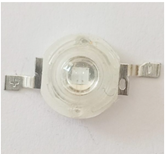
\includegraphics[scale=1]{Chapters/Chapter3/Images/Led5W}
    \end{center}
    \caption{Đèn LED công suất 5W}
    \label{fig:5W}
    \end{figure}
\end{center}

\textbf{Đèn LED công suất 3W:} (Hình~\ref{fig:3W})

Led siêu sáng 3W cho cường độ ánh sáng với góc chiếu tính toán đạt yêu cầu. giá thành của đèn thì là rẻ nhất trong các loại đèn được nhóm đưa ra lựa chọn. Tuy còn điểm yếu chung là góc chiếu nhóm cần tìm và thiết kế chóa phù hợp với đèn.
\begin{center}
    \begin{figure}[ht]
    \begin{center}
     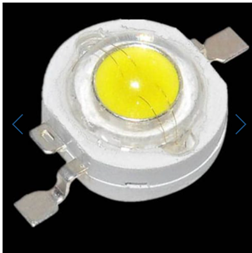
\includegraphics[scale=1]{Chapters/Chapter3/Images/Led3W}
    \end{center}
    \caption{Đèn LED công suất 3W}
    \label{fig:3W}
    \end{figure}
\end{center}

Như vậy qua việc tìm hiểu và kiểm thử các loại đèn thì nhóm chọn được đèn phù hợp với đồ án của nhóm là led siêu sáng 3W với chóa đèn do nhóm tự thiết kế.


\chapter{THI CÔNG HỆ THỐNG ĐIỆN}
\section{Các thiết bị điện}

\subsection{Tổng quan về các phần tử điện}
Để hệ thống hoạt động được luôn cần phần điện. Hệ thống điện chịu trách nhiệm cung cấp nguồn điện, điều khiển các thiết bị trong kết cấu máy như động cơ, driver.
\begin{center}
	\begin{figure}[ht]
	\begin{center}
		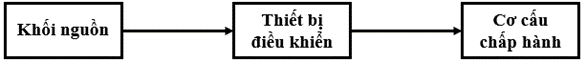
\includegraphics[scale=1]{Chapters/Chapter4/Images/Sodokhoidien}
	\end{center}
	\caption{Sơ đồ các khối trong hệ thống điện}
	\label{fig:sodokhoidien}
	\end{figure}
\end{center}

\subsection{Khối nguồn}
Khối nguồn là bộ phận cung cấp năng lượng cho toàn bộ hệ thống điện trong hệ thống. Để các bóng đèn và động cơ hoạt động ổn định nên nguồn cấp phải đảm bảo điều kiện điện áp và dòng điện luôn ổn định.

Ta lựa chọn nguồn tổ ong.
\begin{figure}[htp]
	\centering
	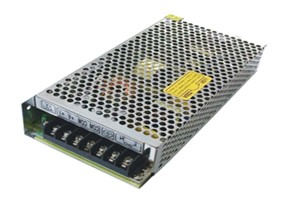
\includegraphics[scale=1]{Chapters/Chapter4/Images/Nguontoong}
	\caption{Nguồn tổ ong}
	\label{fig:Nguontoong}
\end{figure}

Để lựa chọn bộ nguồn phù hợp, phải chú ý đến các thiết bị sử dụng trong mạch điện. Dựa vào thông số về điện áp và dòng điện yêu cầu trên các linh kiện điện để có thể lựa chọn nguồn nuôi thích hợp. Dưới đây là một số linh kiện điện tử và điện áp yêu cầu của các linh kiện đó:
\begin{table}[H]
\centering
\begin{tabular}{|c|c|c|}
\hline 
Linh kiện & Số lượng & Thông số nguồn cấp \\ 
\hline 
LED công suất 3W & 12 & $ 4.2V $ \\ 
\hline 
Driver TB6600 & 3 & $ 12V $ \\ 
\hline 
Động cơ bước & 3 & $ 12V $ \\ 
\hline 
Module L298N & 4 & $ 12V $ \\ 
\hline 
TCA9548A & 1 & $ 5V $ \\ 
\hline 
PCA9685 & 1 & $ 5V $ \\ 
\hline 
\end{tabular} 
\caption{Thông số nguồn cấp cần thiết của các phần tử điện}
\label{tab:nguoncap}
\end{table}

Các thiết bị điện trong máy có dải điện áp hoạt động từ $ 3.8V \sim 12V $.

Cường độ dòng điện cần thiết cho bóng đèn hoạt động: $ 0.789A \times 12 = 9.47(A) $

Cường độ dòng điện cần thiết cho 3 động cơ STEP: $ 0.5A \times 3 = 1.5(A) $

Tổng cường độ dòng điện định mức cần thiết để hệ thống hoạt động bình thường: 
\begin{align*}
9.47A + 1.5A \approx 11A
\end{align*} 

Bộ nguồn được chọn cần có điện áp cung cấp $ 12V $ và dòng điện định mức lớn hơn $ 11A $. Để thuận lợi cho việc nâng cấp hệ thống điện sau này và đảm bảo hệ thống điện hoạt động tốt nhất ta lựa chọn nguồn tổ ong $ 12V30A $

\subsection{Động cơ bước}
Động cơ bước (stepper motor) là một loại động cơ điện có nguyên lý và ứng dụng khác biệt với đa số các động cơ điện thông thường. Chúng thực chất là một động cơ đồng bộ dùng để biến đổi các tín hiệu điều khiển dưới dạng các xung điện rời rạc kế tiếp nhau thành các chuyển động góc quay hoặc các chuyển động của rôto có khả năng cố định rôto vào các vị trí cần thiết.

Động cơ bước không quay theo cơ chế thông thường, chúng quay theo từng bước nên có độ chính xác rất cao về mặt điều khiển. Chúng làm việc nhờ các bộ chuyển mạch điện tử đưa các tín hiệu điều khiển vào stato theo thứ tự và một tần số nhất định. Tổng số góc quay của rôto tương ứng với số lần chuyển mạch, cũng như chiều quay và tốc độ quay của rôto phụ thuộc vào thứ tự chuyển đổi và tần số chuyển đổi.

\begin{figure}[htp]
\centering
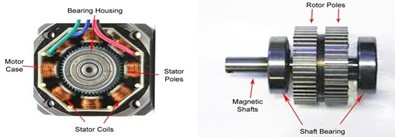
\includegraphics[scale=1]{Chapters/Chapter4/Images/Cautaodongcobuoc.jpg}
\caption{Cấu tạo động cơ bước}
\label{fig:cautaodongcobuoc}
\end{figure}

\subsection{Driver cho động cơ bước}
Một bộ phận không thể thiếu trong điều khiển động cơ bước đó là driver. Driver như là một mạch phân phối xung cho động cơ, làm nhiệm vụ cấp điện cho động cơ bước hoạt động. Có 2 loại driver được xử dụng khá nhiều trong thị trường hiện tại đó là : TB6600 và A4988.

\begin{figure}[ht]
\subfloat[Driver TB6600]
  {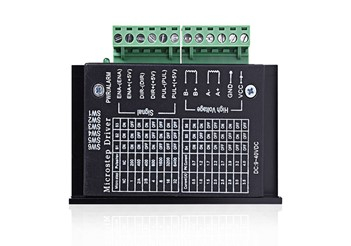
\includegraphics[width=.6\linewidth]{Chapters/Chapter4/Images/DriverTB6600}}\hfill
\subfloat[Driver A4988]
  {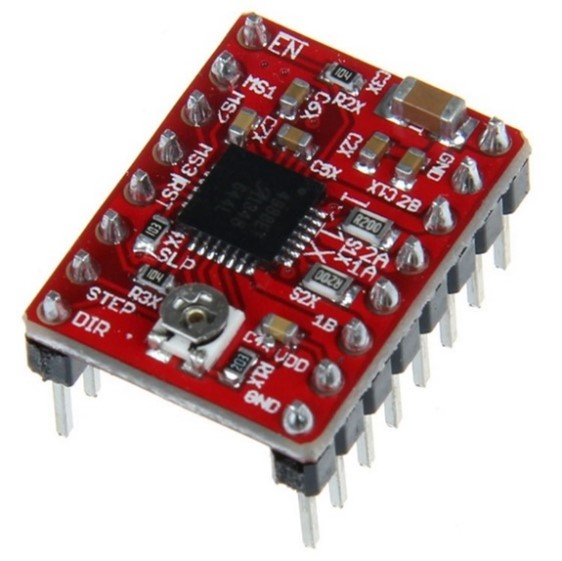
\includegraphics[width=.4\linewidth]{Chapters/Chapter4/Images/DriverA4988}}
\caption{Một số driver cho động cơ bước}
\label{fig:2drivermotor}
\end{figure}

\begin{table}
\centering
\begin{tabular}{|c|c|c|}
\hline 
 & TB6600 & A4988 \\ 
\hline 
Dòng điện ngõ ra & $ 0.5A-4A $ & $ 0.5 - 2A $ \\ 
\hline 
Vi bước nhỏ nhất & $ 1/64 $ & $ 1/16 $ \\ 
\hline 
Điện áp điều khiển & $ 3.3V - 24V $ & $ 0.3V - 5.5V $ \\ 
\hline 
Nguồn cấp cho driver & $ 9V - 42V $ & $ 8V - 35V $ \\ 
\hline 
Bảo vệ quá nhiệt & Có & Có \\ 
\hline 
Bảo vệ ngắn mạch & Có & Không \\ 
\hline 
Kích thước & $ 96 \times 71 \times 37 (mm) $ & $ 5 \times 5 \times 0.9 (mm) $ \\ 
\hline 
Giá thành & 140.000VND & 25.000VND \\ 
\hline 
\end{tabular} 
\caption{Bảng so sánh driver TB6600 và A4988}
\label{tab:sosanhdriver}
\end{table}

Từ Bảng \ref{tab:sosanhdriver}, ta thấy tuy giá thành cao hơn, nhưng driver TB6600 có độ phân giải bước cao hơn, dòng điện điều khiển ngõ ra cũng lớn hơn đồng nghĩa với việc TB6600 sẽ điều khiển vị trí chính xác hơn và động cơ sẽ có momen lớn hơn. Vì thế, trong đồ án này ta sử dụng driver TB6600.

Thông số kỹ thuật:
\begin{itemize}
\item IC Driver: TB6600HQ/HG Single-chip bipolar sinusoidal micro-step stepping motor driver, công nghệ mới nhất BiCD 0.13nm.
\item Nguồn cấp tối đa: 40VDC.
\item Dòng cấp $IIN\_MAX = 5.0A$ và  dòng ra $IOUT\_MAX = 4$.
\item Độ phân giải: 1/1, 1/2, 1/4, 1/8, 1/16, 1/32 và 1/64.
\item Kích thước: 96 x 57 x 35mm.
\end{itemize}

Cách kết nối:
\begin{itemize}
\item DC+: Nối với nguồn điện từ 9 - 40VDC
\item DC- : Điện áp (-) âm của nguồn
\item A+ và A -: Nối vào cặp cuộn dây của động cơ bước
\item B+ và B- : Nối với cặp cuộn dây còn lại của động cơ
\item PUL+: Tín hiệu cấp xung điều khiển tốc độ (+5V) từ BOB cho M6600
\item PUL-: Tín hiệu cấp xung điều khiển tốc độ (-) từ BOB cho M6600
\item DIR+: Tín hiệu cấp xung đảo chiều (+5V) từ BOB cho M6600
\item DIR-: Tín hiệu cấp xung đảo chiều (-) từ BOB cho M6600
\item ENA+ và ENA -: khi cấp tín hiệu cho cặp này động cơ sẽ không có lực momen giữ và quay nữa
\item Có thể đấu tín hiệu dương (+) chung hoặc tín hiệu âm (-) chung.
\end{itemize}


\subsection{Mạch cầu H đầy đủ L298N}
\begin{figure}
\centering
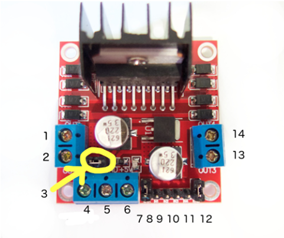
\includegraphics[scale=1]{Chapters/Chapter4/Images/L298N}
\caption{Module L298N}
\label{fig:L298N}
\end{figure}

Thông số kỹ thuật:
\begin{itemize}
\item Driver: L298N tích hợp hai mạch cầu H
\item Điện áp điều khiển: $+5V \sim +12V$
\item Dòng tối đa cho mỗi cầu H là: 2A
\item Điện áp của tín hiệu điều khiển: $ +5V \sim +7V $
\item Dòng của tín hiệu điều khiển : $ 0 \sim 36mA $
\item Công suất hao phí : $ 20W $ (khi nhiệt độ $ T = 75^{\circ}C $)
\item Nhiệt độ bảo quản : $ -25^{\circ}C \sim +130^{\circ}C $
\end{itemize}

Các chân tín hiệu quan trọng:
\begin{itemize}
\item 3: 12V jumper, tháo jumper ra nếu sử dụng nguồn trên 12V. Jumper này dùng để cấp nguồn cho IC ổn áp tạo ra nguồn 5V nếu nguồn trên 12V sẽ làm cháy IC nguồn.
\item 4: Cắm dây nguồn cung cấp điện áp cho motor vào đây từ 6V đến 35V.
\item 5: Cắm chân GND của nguồn vào đây.
\item 6: Ngõ ra nguồn 5V, nếu jumper đầu vào không rút ra.
\item 7: Chân Enable , chân này dùng để cấp xung PWM nếu dùng VDK thì rút jumper ra và cắm chân PWM vào đây.
\item 8, 9, 10, 11: lần lượt là các chân IN1, IN2, IN3, IN4.
\item 12: Chân Enable , chân này dùng để cấp xung PWM nếu dùng VDK thì rút jumper ra và cắm chân PWM vào đây.
\end{itemize}

\subsection{Kit STM32F411 - Discovery}
Thông số kỹ thuật:
\begin{itemize}
\item Bộ điều khiển STM32F411VET6 có 512KB bộ nhớ Flash, 128KB RAM trong gói LQFP100.
\item Cấp nguồn : Thông qua bus USB hoặc cấp điện áp 5V từ bên ngoài.
\item IC L3GD20: Cảm biến chuyển động ST MEMS 3-trục, đầu ra kĩ thuật số.
\item IC LSM303DLHC: Hệ thống ST MEMS trong hệ thống bao gồm bộ cảm biến gia tốc tuyến tính kỹ thuật số 3D và cảm biến từ tính số 3 chiều
\item IC MP45DT02: Bộ cảm biến âm thanh ST MEMS, micro kỹ thuật số.
\item IC CS43L22 : âm thanh DAC với trình điều khiển loa lớp tích hợp D.
\end{itemize}

\begin{figure}[ht]
\centering
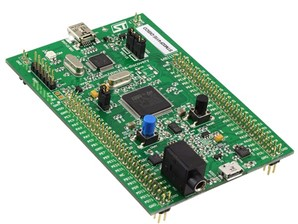
\includegraphics[scale=1]{Chapters/Chapter4/Images/STM32F4.jpg}
\caption{Kit STM32F411 Discovery}
\label{fig:stm32f4}
\end{figure}

\subsection{Module mở rộng giao tiếp I2C 8 kênh TCA9548A}
Thông số kỹ thuật:
\begin{itemize}
\item Điện áp hoạt động: 1.65 – 5.5VDC
\item Số kênh mở rộng: 8 kênh
\item Giao tiếp I2C, địa chỉ chọn được từ 0x70 đến 0x77
\item Điện áp giao tiếp: 1.8, 2.5, 3.3, 5VDC
\item Tần số hoạt động: 0 – 400kHz
\end{itemize}

\begin{figure}
\centering
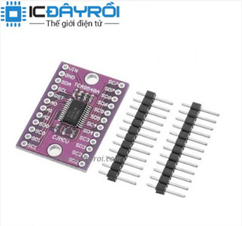
\includegraphics[scale=1]{Chapters/Chapter4/Images/TCA}
\caption{Module TCA9548A}
\label{fig:tca}
\end{figure}


\subsection{PCA9685}
\begin{figure}[htp]
	\centering
	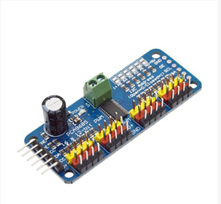
\includegraphics[scale=1]{Chapters/Chapter4/Images/PCA.png}
	\caption{Module PCA9685}
	\label{fig:C4PCA}
\end{figure}
Thông số kỹ thuật:
\begin{itemize}
\item Mạch điều khiển 16 Chanel PWM PCA9685
\item IC chính: PCA9685
\item Điện áp sử dụng: $2.3 \sim 5.5VDC$.
\item Số kênh PWM: 16 kênh, tần số: $40 \sim 1000Hz$
\item Độ phân giải PWM: 12bit.
\item Giao tiếp: I2C (chấp nhận mức Logic TTL $ 3 \sim 5VDC$)
\item Kích thước: $ 62.5mm \times 25.4mm \times 3mm $
\end{itemize}


\subsection{LED công suất 3W}
\begin{figure}[htp]
	\centering
	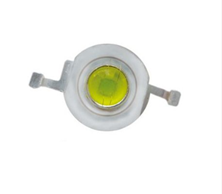
\includegraphics[scale=1]{Chapters/Chapter4/Images/Led3W.png}
	\caption{LED công suất 3W}
	\label{fig:C43W}
\end{figure}
Thông số kỹ thuật:
\begin{itemize}
\item Công suất tiêu thụ 3W
\item Điện áp hoạt động : 3.5-4V
\item Dòng tiêu thụ: 600-750mA
\item Độ sáng : 180LM-200LM
\item Nhiệt độ hoạt động: $ -20^{\circ}C \sim 60^{\circ}C $ \end{itemize}

\subsection{Cảm biến ánh sáng}
Cảm biến cường độ ánh sáng GY-30 BH1750FVI là một cảm biến ánh sáng kỹ thuật số. Gồm một linh kiện điện tử IC cảm biến ánh sáng cho giao tiếp I2C. IC này là thích hợp nhất để nhận diện các dữ liệu ánh sáng xung quanh cho việc điều chỉnh màn hình LCD và bàn phím đèn nền sức mạnh của điện thoại di động. Nó có thể phát hiện nhiều ở độ phân giải cao (1-65535 lx).
\begin{figure}[ht]
	\centering
	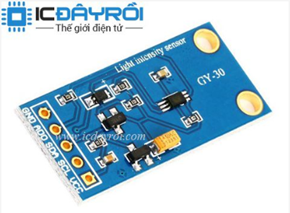
\includegraphics[scale=1]{Chapters/Chapter4/Images/Cambien.png}
	\caption{Cảm biến ánh sáng GY-30 BH1750}
	\label{fig:Cambiengy}
\end{figure}

Thông số kỹ thuật:
\begin{itemize}
\item Module cảm biến cường độ sáng sử dụng chíp BH1750FVI.
\item Điện áp cung cấp: $ 3V - 5V $.
\item Phạm vi phát hiện sáng: $ 0 - 65535 lux $.
\item Cảm biến sử dụng bộ chuyển đổi ADC 16 bit. Tín hiệu đầu ra là tín hiệu số.
\item Giao tiếp với MCU theo chuẩn I2C.
\end{itemize}

\section{Sơ đồ kết nối}

\subsection{Sơ đồ kết nối tổng quát}
Sơ đồ nguyên lý: Hình~\ref{fig:C4Sodotongquat}.

Sơ đồ thực tế: Hình~\ref{fig:C4Sodothucte}.

\begin{figure}[htp]
	\centering
	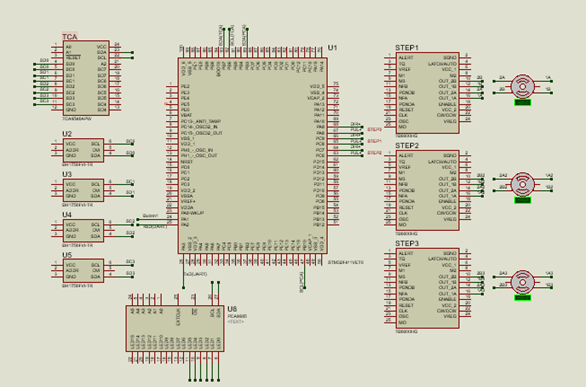
\includegraphics[scale=1]{Chapters/Chapter4/Images/Sodonguyenlytongquat.png}
	\caption{Sơ đồ nguyên lý tổng quát}
	\label{fig:C4Sodotongquat}
\end{figure}
\begin{figure}[htp]
	\centering
	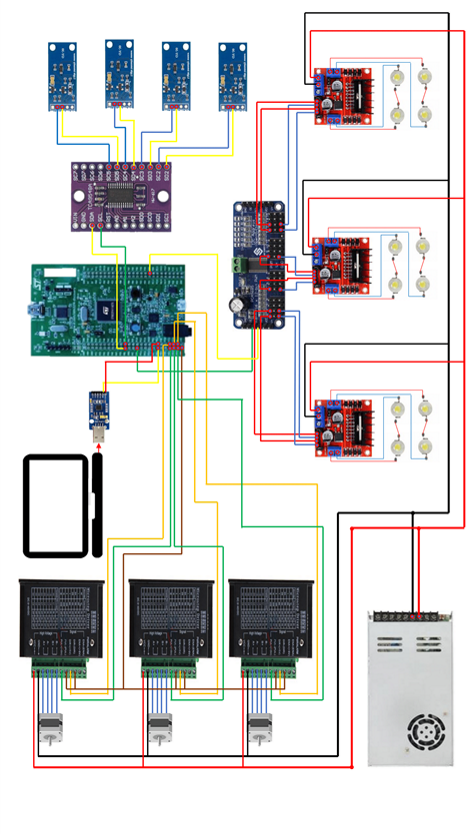
\includegraphics[scale=1]{Chapters/Chapter4/Images/Sodoketnoithucte.png}
	\caption{Sơ đồ kết nối điện thực tế}
	\label{fig:C4Sodothucte}
\end{figure}

\subsection{Sơ đồ kết nối đèn và module L298N}
Sơ đồ nguyên lý: Hình~\ref{fig:C4NLDenL298N}.

Sơ đồ thực tế: Hình~\ref{fig:C4RealDenL298N}.
\begin{figure}[htp]
	\centering
	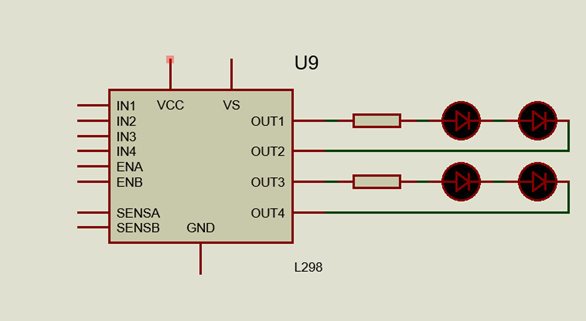
\includegraphics[scale=1]{Chapters/Chapter4/Images/DenL298N.png}
	\caption{Sơ đồ nguyên lý kết nối đèn với module L298N}
	\label{fig:C4NLDenL298N}
\end{figure}
\begin{figure}[htp]
	\centering
	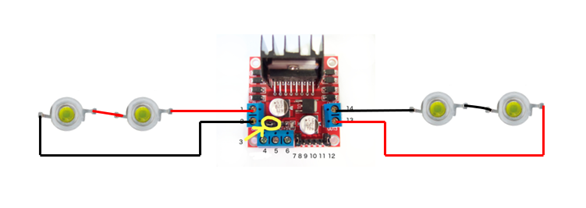
\includegraphics[scale=1]{Chapters/Chapter4/Images/RealDenL298N.png}
	\caption{Sơ đồ kết nối thực tế đèn với module L298N}
	\label{fig:C4RealDenL298N}
\end{figure}

\subsection{Sơ đồ kết nối Driver TB6600 với động cơ bước}
Sơ đồ nguyên lý: Hình~\ref{fig:C4NLDriverDC}.

Sơ đồ thực tế: Hình~\ref{fig:C4RealDriverDC}.

\begin{figure}[htp]
	\centering
	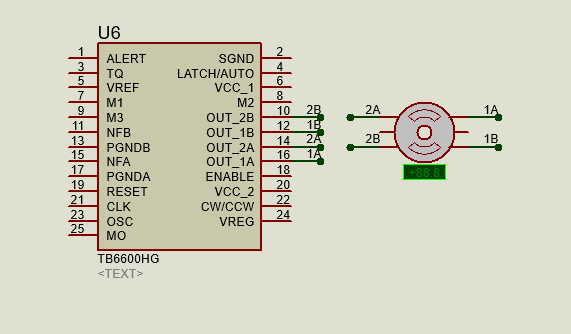
\includegraphics[scale=1]{Chapters/Chapter4/Images/DriverDongco.png}
	\caption{Sơ đồ nguyên lý kết nối Driver và động cơ}
	\label{fig:C4NLDriverDC}
\end{figure}
\begin{figure}[htp]
	\centering
	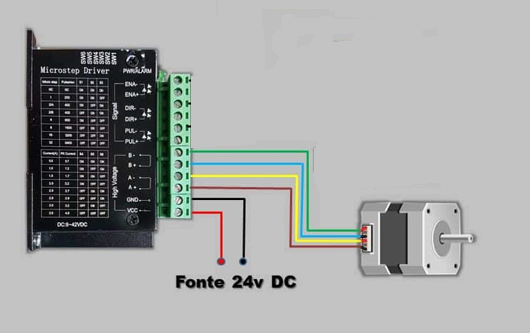
\includegraphics[scale=1]{Chapters/Chapter4/Images/RealDriverDongco.png}
	\caption{Sơ đồ kết nối thực tế Driver và động cơ}
	\label{fig:C4RealDriverDC}
\end{figure}


\chapter{ĐIỀU KHIỂN VÀ LẬP TRÌNH}
\section{Tổng quan về phần điều khiển}
\subsection{Sơ đồ khối hệ thống điều khiển}
\begin{figure}[htp]
	\centering
	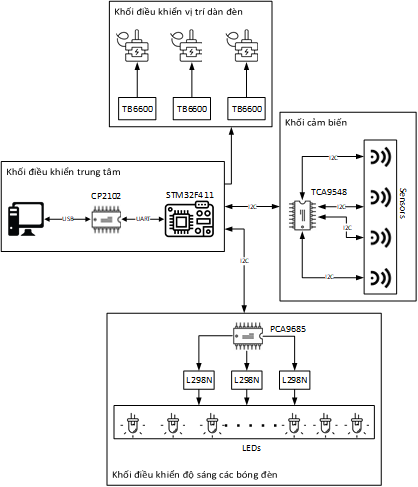
\includegraphics[scale=1]{Chapters/Chapter5/Images/Sodokhoihethong.png}
	\caption{Sơ đồ khối hệ thống điều khiển}
	\label{fig:C5Sodokhoihethong}
\end{figure}

\subsection{Khối điều khiển trung tâm}
\begin{itemize}
\item PC: dùng 1 phần mềm giao diện để gửi tín hiệu điều khiển xuống VĐK và hiển thị dữ liệu do VĐK trả về.
\item VĐK STM32F4: thực hiện các tác vụ chính của hệ thống: truyền nhận tín hiệu I2C với các module, xuất tín hiệu logic tới driver động cơ bước.
\item Module USB to UART CP2102: chuyển đổi giao tiếp từ USB để PC và VĐK có thể giao tiếp với nhau qua chuẩn giao tiếp UART.
\end{itemize}
\begin{figure}[htp]
	\centering
	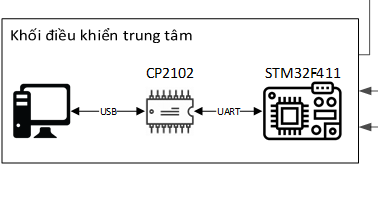
\includegraphics[scale=1]{Chapters/Chapter5/Images/Khoidieukhientrungtam.png}
	\caption{Khối điều khiển trung tâm}
	\label{fig:C5central}
\end{figure}

\subsection{Khối cảm biến}
\begin{figure}[htp]
	\centering
	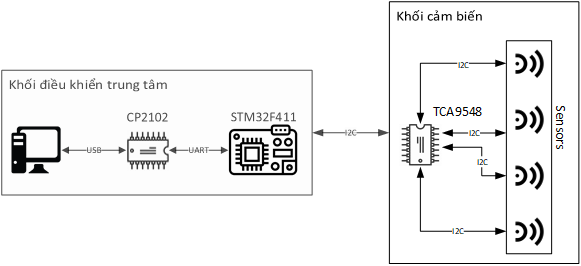
\includegraphics[scale=1]{Chapters/Chapter5/Images/KhoiSensor.png}
	\caption{Khối cảm biến}
	\label{fig:C5Sensor}
\end{figure}
\begin{itemize}
\item Module TCA9548: mở rộng kênh I2C, khuếch đại tín hiệu trên 2 đường dẫn SCL và SDA.
\item Sensors: các module cảm biến GY-30 BH1750. Đo lường cường độ ánh sáng và gửi về VĐK bằng chuẩn giao tiếp I2C.
\end{itemize}

\subsection{Khối điều khiển vị trí các dàn đèn}
\begin{figure}[htp]
	\centering
	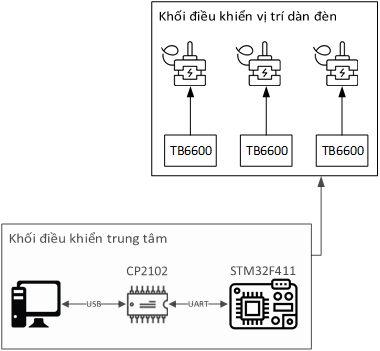
\includegraphics[scale=1]{Chapters/Chapter5/Images/Khoidieukhienlocation.png}
	\caption{Khối điều khiển vị trí các dàn đèn}
	\label{fig:C5Khoidieukhienvitridanden}
\end{figure}
\begin{itemize}
\item Các module TB6600: Nhận xung điều khiển từ VĐK và điều khiển các động cơ quay theo xung điều khiển.
\item Động cơ bước: thông qua bộ truyền đai kéo các dàn đèn để điều khiển dàn đèn tới vị trí mong muốn.
\end{itemize}

\subsection{Khối điều khiển độ sáng các bóng đèn}
\begin{figure}[htp]
	\centering
	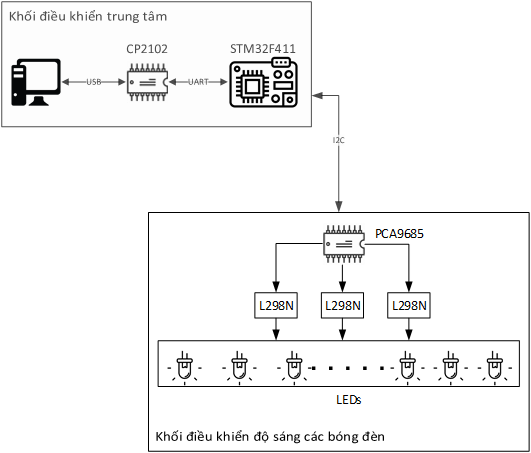
\includegraphics[scale=1]{Chapters/Chapter5/Images/KhoidieukhienLED.png}
	\caption{Khối điều khiển độ sáng các bóng đèn}
	\label{fig:C5KhoidieukhienLED}
\end{figure}
\begin{itemize}
\item PCA9685: Xuất xung PWM để điều khiển độ sáng các bóng đèn.
\item L298N: Nhận xung PWM từ PCA9685 để điều khiển độ sáng bóng đèn lấy nguồn từ bộ nguồn 12V.
\item Bóng đèn LED: Chiếu sáng cho mô hình.
\end{itemize}
\clearpage

\section{Lập trình các chức năng Manual}
\subsection{Lưu đồ giải thuật chương trình điều khiển}
\begin{figure}[H]
	\centering
	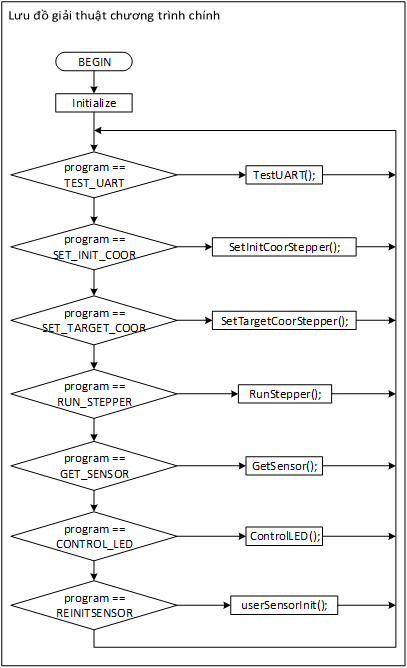
\includegraphics[scale=1]{Chapters/Chapter5/Images/Luudogiaithuatmain.png}
	\caption{Lưu đồ giải thuật chương trình chính}
	\label{fig:C5main}
\end{figure}
\begin{figure}[ht]
	\centering
	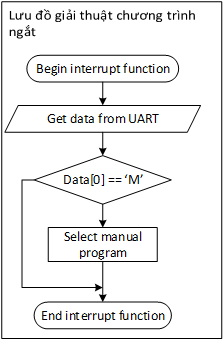
\includegraphics[scale=1]{Chapters/Chapter5/Images/Luudogiaithuatinterrupt.png}
	\caption{Lưu đồ giải thuật chương trình ngắt}
	\label{fig:C5interrupt}
\end{figure}

\subsection{Đọc dữ liệu từ cảm biến}
Một cảm biến ánh sáng GY-30 BH1750 chỉ có thể cài đặt được 2 địa chỉ I2C là “1011100” (0x5C) và “0100011” (0x23). Như vậy 1 kênh I2C chỉ có thể kết nối được tối đa 2 cảm biến. Vi điều khiển STM32F411VETx chỉ có 3 kênh I2C trong khi số cảm biến cần kết nối rất nhiều (16 cảm biến), nên nhóm dùng thêm module tăng số kênh I2C TCA9548A, mở rộng từ 1 kênh I2C lên 8 kênh I2C.

Nhà sản xuất chỉ có sẵn thư viện cho BH1750 và TCA9548A cho dòng VDK  Atmega328P. Vì thế, nhóm phải tự viết lại thư viện riêng dùng bộ thư viện HAL cho dòng VDK STM32F4.

\textbf{Module TCA9548A:}

\textbf{\textit{Địa chỉ I2C:}}
\begin{figure}[H]
	\centering
	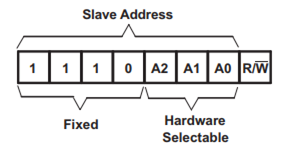
\includegraphics[scale=1]{Chapters/Chapter5/Images/AddressTCA}
	\caption{Địa chỉ I2C của module TCA9548A}
	\label{fig:C5AddressTCA}
\end{figure}

Khi 3 chân A0, A1, A2 trên module được thả nổi thì module sẽ có địa chỉ I2C là 0b1110000 hay 0x70.

\textbf{\textit{Gửi data cho module:}}
\begin{figure}[H]
	\centering
	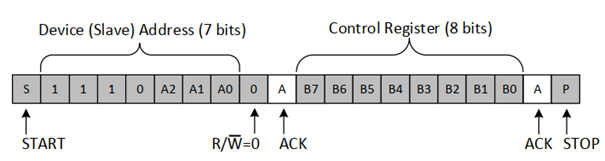
\includegraphics[scale=0.9]{Chapters/Chapter5/Images/SendDataTCA.png}
	\caption{Quy cách gửi data cho module TCA9548A}
	\label{fig:C5SendDataTCA}
\end{figure}

\textbf{\textit{Đọc dữ liệu từ module:}}
\begin{figure}[H]
	\centering
	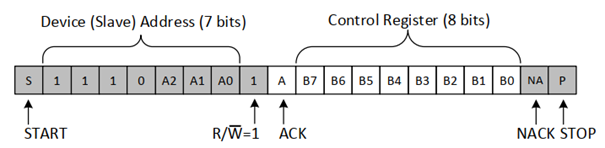
\includegraphics[scale=0.9]{Chapters/Chapter5/Images/ReadDataTCA.png}
	\caption{Quy cách đọc data từ module TCA9548A}
	\label{fig:C5ReadDataTCA}
\end{figure}

\textbf{\textit{Bảng định nghĩa hàm dựa trên control register:}}
\begin{figure}[H]
	\centering
	\includegraphics[scale=1]{Chapters/Chapter5/Images/ControlRegisterTCA.png}
	\caption{Bảng định nghĩa hàm dựa trên Control Register của TCA9548A}
	\label{fig:C5ControlRegisterTCA}
\end{figure}

\textbf{Thư viện cho module TCA9548A}
\begin{lstlisting}
\\ TCA9548A_Driver.h
#ifndef TCA9548_H_
#define TCA9548_H_

#include "main.h"
#include "stm32f4xx_hal_i2c.h"

#define TCA_ADDRESS (0x70 << 1)

typedef enum {
    TCA9548A_OK = 0,
    TCA9548A_ERROR = 1
} TCA9548A_STATUS;

typedef struct TCA9548_Driver {
    I2C_HandleTypeDef *I2C_channel;
    uint8_t Address;
} TCA9548A_HandleTypeDef;

TCA9548A_STATUS TCA9548A_Init(TCA9548A_HandleTypeDef *htca9548a, I2C_HandleTypeDef *hi2c, uint16_t address);
TCA9548A_STATUS TCA9548A_SelectSingleChannel(TCA9548A_HandleTypeDef *htca9548a, uint8_t channel);
TCA9548A_STATUS TCA9548A_SelectMultiChannel(TCA9548A_HandleTypeDef *htca9548a, uint8_t channel);
uint8_t TCA9548A_ReadStatus(TCA9548A_HandleTypeDef *htca9548a);
TCA9548A_STATUS TCA9548A_DisableAllChannel(TCA9548A_HandleTypeDef *htca9548a);

#endif
\end{lstlisting}

\begin{lstlisting}
\\ TCA9548A_Driver.c
#include "TCA9548A_Driver.h"

/*
 * @brief Initialize
 * @param htca9548a Pointer to a TCA9548A_HandleTypeDef
 * @param hi2c Pointer to a I2C_HandleTypeDef structure that contains
 *               the configuration information for the specified I2C.
 * @param address Target BH1750 device address. The device 7 bits address value in datasheet must
 *                be shifted to the left before calling by I2C function.
 * @retval TCA9548A Status
 */
TCA9548A_STATUS TCA9548A_Init(TCA9548A_HandleTypeDef *htca9548a, I2C_HandleTypeDef *hi2c, uint16_t address) {
    htca9548a->I2C_channel = hi2c;
    htca9548a->Address = address;

    if (TCA9548A_OK == TCA9548A_DisableAllChannel(htca9548a)) {
        return TCA9548A_OK;
    }
    return TCA9548A_ERROR;
}

/*
 * @brief Initialize
 * @param htca9548a Pointer to a TCA9548A_HandleTypeDef
 * @param channel From 0 to 7, is channel 0 to channel 7 on TCA9548A
 * @retval TCA9548A Status
 */
TCA9548A_STATUS TCA9548A_SelectSingleChannel(TCA9548A_HandleTypeDef *htca9548a, uint8_t channel) {
    if (channel > 7) {
        return TCA9548A_ERROR;
    }
    uint8_t tmp = (1 << channel);
    if (HAL_OK == HAL_I2C_Master_Transmit(htca9548a->I2C_channel, htca9548a->Address, &tmp, 1, 10)) {
        return TCA9548A_OK;
    }
    return TCA9548A_ERROR;
}

/*
 * @brief Initialize
 * @param htca9548a Pointer to a TCA9548A_HandleTypeDef
 * @param channel This have 8 bit to choose which channel is selected.
 *                Ex: channel 0, 3, 5 is selected, channel = 0b00101001 = 0x29 
 * @retval TCA9548A Status
 */
TCA9548A_STATUS TCA9548A_SelectMultiChannel(TCA9548A_HandleTypeDef *htca9548a, uint8_t channel) {
    if (HAL_OK == HAL_I2C_Master_Transmit(htca9548a->I2C_channel, htca9548a->Address, &channel, 1, 10)) {
        return TCA9548A_OK;
    }
    return TCA9548A_ERROR;
}

uint8_t TCA9548A_ReadStatus(TCA9548A_HandleTypeDef *htca9548a) {
    uint8_t tmp;
    if (HAL_OK == HAL_I2C_Master_Receive(htca9548a->I2C_channel, htca9548a->Address, &tmp, 1, 10)) {
        return tmp;
    }
    return 0;
}

TCA9548A_STATUS TCA9548A_DisableAllChannel(TCA9548A_HandleTypeDef *htca9548a) {
    uint8_t tmp = 0x00;
    if (HAL_OK == HAL_I2C_Master_Transmit(htca9548a->I2C_channel, htca9548a->Address, &tmp, 1, 10)) {
        return TCA9548A_OK;
    }
    return TCA9548A_ERROR;
}
\end{lstlisting}
\clearpage

\textbf{Module GY-30 BH1750}

\textbf{\textit{Địa chỉ I2C}}

Khi chân ADDR của module có tín hiệu mức cao $(\geq 0.7VCC)$ thì module có địa chỉ là: 0b1011100 hay 0x5C, ngược lại module sẽ có địa chỉ là 0b0100011 hay 0x23.

\textbf{\textit{Gửi data cho module:}}
\begin{figure}[H]
	\centering
	\includegraphics[scale=0.9]{Chapters/Chapter5/Images/SendDataGY30.png}
	\caption{Gửi data cho module BH1750}
	\label{fig:C5SendDataGY30}
\end{figure}

\textbf{\textit{Đọc data từ module:}}
\begin{figure}[H]
	\centering
	\includegraphics[scale=0.9]{Chapters/Chapter5/Images/ReadDataGY30.png}
	\caption{Đọc data từ module BH1750}
	\label{fig:C5ReadDataGY30}
\end{figure}

\textbf{\textit{Bảng mã điều khiển:}}
\begin{figure}[H]
	\centering
	\includegraphics[scale=0.9]{Chapters/Chapter5/Images/OpecodeGY30.png}
	\caption{Bảng mã điều khiển của module BH1750}
	\label{fig:C5OpecodeGY30}
\end{figure}

\textbf{Thư viện cho module GY-30 BH1750:}
\begin{lstlisting}
\\ BH1750_Driver.h
#ifndef BH1750_H_
#define BH1750_H_

/* Include ------------ */
#include "stm32f4xx_hal.h"

#define BH1750_ADDRESS_HIGH        (0x5C<<1)
#define BH1750_ADDRESS_LOW         (0x23<<1)

#define BH1750_POWER_DOWN          0x00
#define BH1750_POWER_ON            0x01
#define BH1750_RESET               0x07

#define BH1750_DEFAULT_MTREG       69
#define BH1750_CONVERSION_FACTOR   1.2

typedef enum {
    BH1750_OK    = 0,
    BH1750_ERROR = 1
} BH1750_STATUS;

typedef enum {
    CONTINUOUS_H_RES_MODE    = 0x10,
    CONTINUOUS_H_RES_MODE2   = 0x11,
    CONTINUOUS_L_RES_MODE    = 0x13,
    ONETIME_H_RES_MODE       = 0x20,
    ONETIME_H_RES_MODE2      = 0x21,
    ONETIME_L_RES_MODE       = 0x23
} bh1750_mode;

typedef struct BH1750_Driver
{
    I2C_HandleTypeDef *I2C_channel;
    uint16_t Address;

} BH1750_HandleTypeDef;

BH1750_STATUS BH1750_Init(BH1750_HandleTypeDef *hbh1750, I2C_HandleTypeDef *hi2c, uint16_t Address);
BH1750_STATUS BH1750_Reset(BH1750_HandleTypeDef *hbh1750);
BH1750_STATUS BH1750_PowerState(BH1750_HandleTypeDef *hbh1750, uint8_t PowerOn);
BH1750_STATUS BH1750_SetMtreg(BH1750_HandleTypeDef *hbh1750, uint8_t Mtreg);
BH1750_STATUS BH1750_SetMode(BH1750_HandleTypeDef *hbh1750, bh1750_mode Mode);
BH1750_STATUS BH1750_TriggerManualConversion(BH1750_HandleTypeDef *hbh1750);
BH1750_STATUS BH1750_ReadLight(BH1750_HandleTypeDef *hbh1750, uint16_t *Result);

#endif /* BH1750_H_ */
\end{lstlisting}

\begin{lstlisting}
\\ BH1750_Driver.c
/*
 =======================================================
          ##### How to use this driver #####
 =======================================================
    Set up:
    #1  @ref BH1750_Init()
        Ex: BH1750_Init(&sensor[i], &hi2c1, BH1750_ADDRESS_LOW);
    #2  @ref BH1750_PowerState()
        Ex: BH1750_PowerState(&sensor[i], 1);
    #3  @ref BH1750_SetMode()
        Ex: BH1750_SetMode(&sensor[i], CONTINUOUS_H_RES_MODE);
        
    Let play: Read light @ref BH1750_ReadLight()
    BH1750_ReadLight(&sensor[i], &result[i]);
*/

#include "BH1750_Driver.h"

bh1750_mode     BH1750_Mode;
uint8_t         BH1750_Mtreg;

/*
 * @brief Initialize
 * @param hbh1750 Pointer to a BH1750_HandleTypeDef
 * @param hi2c Pointer to a I2C_HandleTypeDef structure that contains
 *               the configuration information for the specified I2C.
 * @param Address Target BH1750 device address. The device 7 bits address value in datasheet must
 *                be shifted to the left before calling by I2C function.
 * @retval BH1750 Status
 */
BH1750_STATUS BH1750_Init(BH1750_HandleTypeDef *hbh1750, I2C_HandleTypeDef *hi2c, uint16_t Address) {
    hbh1750->I2C_channel = hi2c;
    hbh1750->Address = Address;
    if(BH1750_OK == BH1750_Reset(hbh1750))
    {
        if(BH1750_OK == BH1750_SetMtreg(hbh1750, BH1750_DEFAULT_MTREG)) // Set default value;
            return BH1750_OK;
    }
    return BH1750_ERROR;
}

/* 
 * @brief Reset all registers to default value.
 * @param hbh1750 Pointer to a BH1750_HandleTypeDef
 * @retval BH1750 status
 */
BH1750_STATUS BH1750_Reset(BH1750_HandleTypeDef *hbh1750) {
    uint8_t tmp = BH1750_RESET;
    if (HAL_OK == HAL_I2C_Master_Transmit(hbh1750->I2C_channel, hbh1750->Address, &tmp, 1, 10))
        return BH1750_OK;
    return BH1750_ERROR;
}

/*
 * @brief Set the power state.
 * @param hbh1750 Pointer to a BH1750_HandleTypeDef
 * @param PowerOn
 *          @arg 0: Power down, low current, no active state.
 *          @arg 1: Ready for measurement command. 
 * @retval BH1750 status
 */
BH1750_STATUS BH1750_PowerState(BH1750_HandleTypeDef *hbh1750, uint8_t PowerOn) {
    PowerOn = (PowerOn ? 1 : 0);
    if (HAL_OK == HAL_I2C_Master_Transmit(hbh1750->I2C_channel, hbh1750->Address, &PowerOn, 1, 10))
        return BH1750_OK;
    return BH1750_ERROR;
}

/*
 * @brief Adjust measurement result for influence of optical window. (sensor sensitivity adjusting) 
 * @param hbh1750 Pointer to a BH1750_HandleTypeDef
 * @param Mtreg The modified value of measurement time register. (31 <= Mtreg <=254) (miliseconds)
 * @retval BH1750 status
 */
BH1750_STATUS BH1750_SetMtreg(BH1750_HandleTypeDef *hbh1750, uint8_t Mtreg) {
    HAL_StatusTypeDef retCode;
    if (Mtreg < 31 || Mtreg > 254) {
        return BH1750_ERROR;
    }

    BH1750_Mtreg = Mtreg;

    uint8_t tmp[2];

    tmp[0] = (0x40 | (Mtreg >> 5));     // High bit 01000_MT[7,6,5]
    tmp[1] = (0x60 | (Mtreg & 0x1F));   // Low bit  011_MT[4,3,2,1,0] 

    retCode = HAL_I2C_Master_Transmit(hbh1750->I2C_channel, hbh1750->Address, &tmp[0], 1, 10);
    if (HAL_OK != retCode) {
        return BH1750_ERROR;
    }

    retCode = HAL_I2C_Master_Transmit(hbh1750->I2C_channel, hbh1750->Address, &tmp[1], 1, 10);
    if (HAL_OK == retCode) {
        return BH1750_OK;
    }

    return BH1750_ERROR;
}

/*
 * @brief Set the mode of converting. Look into bh1750_mode enum.
 * @param hbh1750 Pointer to a BH1750_HandleTypeDef
 * @param Mode The mode of converting. This parameter can be one of the bh1750_mode enum values:
 *              @arg CONTINUOUS_H_RES_MODE:  Start measurement at 1lx resolution.
 *                                           Measurement Time is typically 120ms. 
 *              @arg CONTINUOUS_H_RES_MODE2: Start measurement at 0.5lx resolution.
 *                                           Measurement Time is typically 120ms. 
 *              @arg CONTINUOUS_L_RES_MODE:  Start measurement at 4lx resolution. 
 *                                           Measurement Time is typically 16ms. 
 *              @arg ONETIME_H_RES_MODE:     Start measurement at 1lx resolution.
 *                                           Measurement Time is typically 120ms. 
 *                                           It is automatically set to Power Down mode after measurement.
 *              @arg ONETIME_H_RES_MODE2:    Start measurement at 0.5lx resolution.
 *                                           Measurement Time is typically 120ms. 
 *                                           It is automatically set to Power Down mode after measurement.
 *              @arg ONETIME_L_RES_MODE:     Start measurement at 4lx resolution.
 *                                           Measurement Time is typically 16ms. 
 *                                           It is automatically set to Power Down mode after measurement.
 * @retval BH1750 status
 */
BH1750_STATUS BH1750_SetMode(BH1750_HandleTypeDef *hbh1750, bh1750_mode Mode) {
    if(!((Mode >> 4) || (Mode >> 5))) return BH1750_ERROR;
    if((Mode & 0x0F) > 3) return BH1750_ERROR;

    BH1750_Mode = Mode;
    if(HAL_OK == HAL_I2C_Master_Transmit(hbh1750->I2C_channel, hbh1750->Address, &Mode, 1, 10))
        return BH1750_OK;

    return BH1750_ERROR;
}

// BH1750_STATUS BH1750_TriggerManualConversion(uint16_t Address);

/*
 * @brief Read the converted value and calculate the result.
 * @param hbh1750 Pointer to a BH1750_HandleTypeDef
 * @param Result Pointer to your variable for getting result.
 * @retval BH1750 Status
 */
BH1750_STATUS BH1750_ReadLight(BH1750_HandleTypeDef *hbh1750, uint16_t *Result) {
    uint16_t result;
    uint8_t tmp[2];

    if(HAL_OK == HAL_I2C_Master_Receive(hbh1750->I2C_channel, hbh1750->Address, tmp, 2, 10))
    {
        result = (tmp[0] << 8) | (tmp[1]);

        if(BH1750_Mtreg != BH1750_DEFAULT_MTREG)
        {
            result *= (float)((uint8_t)(BH1750_DEFAULT_MTREG) / (float)BH1750_Mtreg);
        }

        if(BH1750_Mode == ONETIME_H_RES_MODE2 || BH1750_Mode == CONTINUOUS_H_RES_MODE2)
        {
            result /= 2.0;
        }

        *Result = result / (float)BH1750_CONVERSION_FACTOR;
        return BH1750_OK;
    }
    return BH1750_ERROR;
}
\end{lstlisting}



Phần chương trình đọc dữ liệu cảm biến trong file main.c:
\begin{lstlisting}
// Variables for Sensor and TCA
TCA9548A_HandleTypeDef i2cHub;
BH1750_HandleTypeDef sensor[4];
char dataSensorMessage[24] = {};
uint16_t dataSensor[4];
uint8_t ret;
void userSensorInit() {
  TCA9548A_Init(&i2cHub, &hi2c1, TCA_ADDRESS);
  for (uint8_t i = 0; i < 4; i++) {
    TCA9548A_SelectSingleChannel(&i2cHub, i);
    BH1750_Init(&sensor[i], &hi2c1, BH1750_ADDRESS_LOW);
    BH1750_PowerState(&sensor[i], 1);
    BH1750_SetMode(&sensor[i], CONTINUOUS_H_RES_MODE);
  }
}
void GetSensor() {
  for (uint8_t i = 0; i < 4; i++) {
    TCA9548A_SelectSingleChannel(&i2cHub, i);
    BH1750_ReadLight(&sensor[i], &dataSensor[i]);

    dataSensorMessage[i*6 + 5] = (i < 3) ? ' ' : '\n';
    dataSensorMessage[i*6 + 4] = dataSensor[i] % 10 + '0';
    dataSensorMessage[i*6 + 3] = dataSensor[i] / 10 % 10 + '0';
    dataSensorMessage[i*6 + 2] = dataSensor[i] / 100 % 10 + '0';
    dataSensorMessage[i*6 + 1] = dataSensor[i] / 1000 % 10 + '0';
    dataSensorMessage[i*6 + 0] = dataSensor[i] / 10000 % 10 + '0';
  }
  HAL_UART_Transmit(&huart2, (uint8_t *)dataSensorMessage, 24, 24);
  program = IDLE;
}
\end{lstlisting}

\subsection{Điều khiển toạ độ các dàn đèn}
Tọa độ của các dàn đèn được điều khiển bởi các động cơ bước sử dụng TB6600 làm driver. 

\textbf{Thư viện cho Driver TB6600:}
\begin{lstlisting}
\\ Stepper_Driver.h
#ifndef STEPPERDRIVER_H_
#define STEPPERDRIVER_H_

#include "stm32f4xx_hal.h"

// Time delay write HIGH and LOW to PIN PULSE in microsecond
#define TdelayON    50
#define TdelayOFF  300

// diameter of pulley (millimeters)
#define DIAMETER 13.2
#define PI        3.14159

// PulTranfer = 200 * stepper->Microstep / Diameter / PI    = 160
#define FACTOR 160

typedef enum {
    STEPPER_OK    = 0,
    STEPPER_ERROR = 1
} STEPPER_STATUS;

typedef struct StepperDriver {
    GPIO_TypeDef* Port;
    uint16_t GPIO_Pin_Dir;
    uint16_t GPIO_Pin_Pulse;
    // uint16_t GPIO_Pin_Enable;
    uint8_t Microstep;
    uint32_t CurrentPulse;
    uint32_t TargetPulse;
} Stepper_HandleTypeDef;

STEPPER_STATUS StepperInit(Stepper_HandleTypeDef *stepper,
                           GPIO_TypeDef* port,
                           uint16_t pin_Dir,
                           uint16_t pin_Pulse,
                           uint8_t microstep,
                           uint16_t currentPos);
STEPPER_STATUS setCurrentPos(Stepper_HandleTypeDef *stepper, uint16_t current);
STEPPER_STATUS setTargetPos(Stepper_HandleTypeDef *stepper, uint16_t target);
STEPPER_STATUS setDirCCW(Stepper_HandleTypeDef *stepper);
STEPPER_STATUS setDirCW(Stepper_HandleTypeDef *stepper);
STEPPER_STATUS runToTarget(Stepper_HandleTypeDef *stepper);

#endif /* STEPPERDRIVER_H_ */
\end{lstlisting}

\begin{lstlisting}
\\ Stepper_Driver.c
/*
 * StepperDriver.c
 *
 *  Created on: Apr 25, 2021
 *      Author: Ice Cream
 *
 *============================================================
 *      HOW TO USE THIS DRIVER
 *============================================================
 *   #1: Khoi tao dong co bang ham @ref StepperInit()
 *   #2: Dat vi tri ban dau bang ham @ref setCurrentPos()
 *   #3: Dat vi tri muon di toi bang ham @ref setTargetPos()
 *   #4: Them ham @ref runToTarget() vao vong lap de dong co se tu dong chay toi vi
 *       da chon.
 *
 */

#include "StepperDriver.h"

/*
 * @brief Initialize
 * @param stepper Pointer to a Stepper Motor
 * @param Port is GPIOx, x is the port (A ... E) you connect the 
 *         direction and pulse pins from the driver to stm32
 * @param microstep specifies the microstep value that in use. (usually 1, 2, 4, 8, 16, 32)
 * @param currentPos specifies the motor's current position 
 * @retval Stepper Status
 */
STEPPER_STATUS StepperInit(Stepper_HandleTypeDef *stepper,
                           GPIO_TypeDef* port,
                           uint16_t pin_Dir,
                           uint16_t pin_Pulse,
                           uint8_t microstep,
                           uint16_t currentPos) {
    stepper->Port           = port;
    stepper->GPIO_Pin_Dir   = pin_Dir;
    stepper->GPIO_Pin_Pulse = pin_Pulse;
    stepper->Microstep      = microstep;
    stepper->CurrentPulse   = currentPos * FACTOR;
    stepper->TargetPulse    = currentPos * FACTOR;

    return STEPPER_OK;
}

STEPPER_STATUS setCurrentPos(Stepper_HandleTypeDef *stepper, uint16_t current) {
    stepper->CurrentPulse = current * FACTOR;
    stepper->TargetPulse = current * FACTOR;
    return STEPPER_OK;
}

STEPPER_STATUS setTargetPos(Stepper_HandleTypeDef *stepper, uint16_t target) {
    stepper->TargetPulse = target * FACTOR;
    return STEPPER_OK;
}

STEPPER_STATUS setDirCCW(Stepper_HandleTypeDef *stepper) {
    HAL_GPIO_WritePin(stepper->Port, stepper->GPIO_Pin_Dir, GPIO_PIN_SET);
    return STEPPER_OK;
}

STEPPER_STATUS setDirCW(Stepper_HandleTypeDef *stepper) {
    HAL_GPIO_WritePin(stepper->Port, stepper->GPIO_Pin_Dir, GPIO_PIN_RESET);
    return STEPPER_OK;
}

__weak void delay_us(uint16_t us)
{
  /* Prevent unused argument(s) compilation warning */
  UNUSED(us);
  /*  TIM2 configure
   *  Clock Source: Internal Clock
   *  Prescaler: 50 - 1
   *  Counter Period: 0xFFFF - 1
   *  Clock Configure: 50MHz
     *  don't forget to add this below USER CODE BEGIN 2
   *  HAL_TIM_Base_Start(&htim2);
   *  Code:
   *  __HAL_TIM_SET_COUNTER(&htim2,0);  // set the counter value a 0
   *  while ((uint16_t)__HAL_TIM_GET_COUNTER(&htim2) < us);
   */
}

STEPPER_STATUS runToTarget(Stepper_HandleTypeDef *stepper) {

    if (stepper->TargetPulse != stepper->CurrentPulse) {
        // convert Position in millimeters to pulses base on microstep
        
        if (stepper->TargetPulse > stepper->CurrentPulse) {
            setDirCCW(stepper);
            HAL_GPIO_WritePin(stepper->Port, stepper->GPIO_Pin_Pulse, GPIO_PIN_SET);
            delay_us(TdelayON);
            HAL_GPIO_WritePin(stepper->Port, stepper->GPIO_Pin_Pulse, GPIO_PIN_RESET);
            delay_us(TdelayOFF);
            stepper->CurrentPulse++;
        }
        else {
            setDirCW(stepper);
            HAL_GPIO_WritePin(stepper->Port, stepper->GPIO_Pin_Pulse, GPIO_PIN_SET);
            delay_us(TdelayON);
            HAL_GPIO_WritePin(stepper->Port, stepper->GPIO_Pin_Pulse, GPIO_PIN_RESET);
            delay_us(TdelayOFF);
            stepper->CurrentPulse--;
        }
        return STEPPER_ERROR;
    }
    return STEPPER_OK;
}
\end{lstlisting}

Phần điều khiển các động cơ trong file main.c:
\begin{lstlisting}
void SetInitCoorStepper() {
  DecryptData();
  setCurrentPos(&Step0, info[0]);
  setCurrentPos(&Step1, info[1]);
  setCurrentPos(&Step2, info[2]);
  HAL_UART_Transmit(&huart2, InitStepperMessage, sizeof(InitStepperMessage), 1000);
  program = IDLE;
}

void SetTargetCoorStepper() {
  DecryptData();
  setTargetPos(&Step0, info[0]);
  setTargetPos(&Step1, info[1]);
  setTargetPos(&Step2, info[2]);
  keepMotorSafe();
  uint32_t locationStep0 = Step0.TargetPulse / FACTOR;
  uint32_t locationStep1 = Step1.TargetPulse / FACTOR;
  uint32_t locationStep2 = Step2.TargetPulse / FACTOR;
  uint8_t locationMessage[20];
  locationMessage[0] = 'T';
  locationMessage[1] = 'a';
  locationMessage[2] = 'r';
  locationMessage[3] = 'g';
  locationMessage[4] = 'e';
  locationMessage[5] = 't';
  locationMessage[6] = ':';
  locationMessage[7] = ' ';
  // Step0
  locationMessage[10] = locationStep0 % 10 + '0';
  locationMessage[9] = locationStep0 / 10 % 10 + '0';
  locationMessage[8] = locationStep0 / 100 % 10 + '0';
  locationMessage[11] = ' ';
  // Step1
  locationMessage[14] = locationStep1 % 10 + '0';
  locationMessage[13] = locationStep1 / 10 % 10 + '0';
  locationMessage[12] = locationStep1 / 100 % 10 + '0';
  locationMessage[15] = ' ';
  // Step2
  locationMessage[18] = locationStep2 % 10 + '0';
  locationMessage[17] = locationStep2 / 10 % 10 + '0';
  locationMessage[16] = locationStep2 / 100 % 10 + '0';
  locationMessage[19] = '\n';

  HAL_UART_Transmit(&huart2, locationMessage, sizeof(locationMessage), 1000);
  program = RUN_STEPPER;
}

void RunStepper() {
  uint8_t flag = 0;
  if (runToTarget(&Step0) == STEPPER_ERROR) flag = 1;
  if (runToTarget(&Step1) == STEPPER_ERROR) flag = 1;
  if (runToTarget(&Step2) == STEPPER_ERROR) flag = 1;
  if (flag == 0) {
    HAL_UART_Transmit(&huart2, Done, sizeof(Done), 1000);
    program = IDLE;
  }
}
\end{lstlisting}

\subsection{Điều khiển độ sáng của các bóng đèn}
Độ sáng của các bóng đèn được điều khiển bằng module PCA9685. Tuy nhiên do module này chỉ có thể xuất xung PWM với 25mA, 5.5V trong khi bóng đèn sử dụng trong mô hình là đèn công suất với dòng cao. Vì thế nhóm sử dụng thêm module L298N để nhận xung PWM và cấp điện cho đèn.

\textbf{Module PCA9685:}

\textbf{\textit{Địa chỉ I2C:}}
\begin{figure}[H]
	\centering
	\includegraphics[scale=1]{Chapters/Chapter5/Images/AddressPCA.png}
	\caption{Địa chỉ của module PCA9685}
	\label{fig:C5AddressPCA}
\end{figure}

Các chân A0 tới A5 đều đang thả nổi, địa chỉ của module hiện tại là: 0b1000000 hay 0x40. 

\textbf{Cài đặt xung PWM cho 1 channel:}

Module tính toán thời điểm tắt và bật bằng counter với xung clock đầu vào là 27MHz. Các thanh ghi sử dụng (giả sử đối với channel 0):

LED0\_ON\_H, LED0\_ON\_L: 2 byte này lưu trữ thời điểm IC sẽ xuất tín hiệu ra chân PWM lên mức HIGH.

LED0\_OFF\_H, LED0\_OFF\_L: 2 byte này lưu trữ thời điểm IC sẽ xuất tín hiệu ra chân PWM xuống mức LOW.

Ví dụ cách tính giá trị cần ghi vào các thanh ghi trên:
\begin{align*}
&Delay time =  10\% \\
&PWM Duty Cycle = 20\% (LED on time = 20\%, LED off time = 80\%)
\end{align*}

Tính toán: 
\begin{align*}
Delay time = 4096 \times 10\% = 409.6 \approx 410 = 0x19A
\end{align*}

Do counter đếm từ 0 tới 4096 nên $ Delay time = 0x199 $.
\begin{align*}
&LED0\_ON\_H = 0x1, LED0\_ON\_L = 0x99 \\
&LED \; on \; time = 20\% = 819.2 \sim 819 counts \\
&LED \; off \; time = 0x4CC \\
&LED0\_OFF\_H = 0x4,\; LED0\_OFF\_L = 0xCC 
\end{align*}

\textbf{\textit{Gửi data cho module:}}
\begin{figure}[H]
	\centering
	\includegraphics[scale=0.9]{Chapters/Chapter5/Images/SendDataPCA.png}
	\caption{Gửi data cho module PCA9685}
	\label{fig:C5SendDataPCA}
\end{figure}

\begin{lstlisting}
\\ PCA9685_Driver.h
#ifndef PCA9685_H_
#define PCA9685_H_

// include
#include "stm32f4xx_hal.h"

// REGISTER ADDRESSES
#define PCA9685_MODE1       0x00    /**< Mode Register 1 */
#define PCA9685_MODE2       0x01    /**< Mode Register 2 */
#define PCA9685_SUBADR1     0x02    /**< I2C-bus subaddress 1 */
#define PCA9685_SUBADR2     0x03    /**< I2C-bus subaddress 2 */
#define PCA9685_SUBADR3     0x04    /**< I2C-bus subaddress 3 */
#define PCA9685_ALLCALLADR  0x05    /**< LED All Call I2C-bus address */
#define PCA9685_LED0_ON_L   0x06    /**< LED0 on tick, low byte*/
#define PCA9685_LED0_ON_H   0x07    /**< LED0 on tick, high byte*/
#define PCA9685_LED0_OFF_L  0x08    /**< LED0 off tick, low byte */
#define PCA9685_LED0_OFF_H  0x09    /**< LED0 off tick, high byte */

// etc all 16:  LED15_OFF_H 0x45
#define PCA9685_ALLLED_ON_L     0xFA    /**< load all the LEDn_ON registers, low */
#define PCA9685_ALLLED_ON_H     0xFB    /**< load all the LEDn_ON registers, high */
#define PCA9685_ALLLED_OFF_L    0xFC    /**< load all the LEDn_OFF registers, low */
#define PCA9685_ALLLED_OFF_H    0xFD    /**< load all the LEDn_OFF registers,high */
#define PCA9685_PRESCALE        0xFE    /**< Prescaler for PWM output frequency */
#define PCA9685_TESTMODE        0xFF    /**< defines the test mode to be entered */

// MODE1 bits
#define MODE1_ALLCAL    0x01    /**< respond to LED All Call I2C-bus address */
#define MODE1_SUB3      0x02    /**< respond to I2C-bus subaddress 3 */
#define MODE1_SUB2      0x04    /**< respond to I2C-bus subaddress 2 */
#define MODE1_SUB1      0x08    /**< respond to I2C-bus subaddress 1 */
#define MODE1_SLEEP     0x10    /**< Low power mode. Oscillator off */
#define MODE1_AI        0x20    /**< Auto-Increment enabled */
#define MODE1_EXTCLK    0x40    /**< Use EXTCLK pin clock */
#define MODE1_RESTART   0x80    /**< Restart enabled */
// MODE2 bits
#define MODE2_OUTNE_0   0x01    /**< Active LOW output enable input */
#define MODE2_OUTNE_1   0x02    /**< Active LOW output enable input - high impedience */
#define MODE2_OUTDRV    0x04    /**< totem pole structure vs open-drain */
#define MODE2_OCH       0x08  /**< Outputs change on ACK vs STOP */
#define MODE2_INVRT     0x10  /**< Output logic state inverted */

#define PCA9685_I2C_ADDRESS     (0x40<<1)   /**< Default PCA9685 I2C Slave Address */
#define FREQUENCY_OSCILLATOR    25000000    /**< Int. osc. frequency in datasheet */

#define PCA9685_PRESCALE_MIN    3   /**< minimum prescale value */
#define PCA9685_PRESCALE_MAX    255 /**< maximum prescale value */

// Variable
typedef struct PCA9685_Driver {
    I2C_HandleTypeDef *hi2c;
    uint8_t Address;
} PCA9685_HandleTypeDef;

// function
void PCA9685_Init(PCA9685_HandleTypeDef *hpca9685, 
                                    I2C_HandleTypeDef *hi2c,
                                    uint8_t addr,
                                    uint8_t prescale);
void PCA9685_Reset(PCA9685_HandleTypeDef *hpca9685);
void PCA9685_Sleep(PCA9685_HandleTypeDef *hpca9685);
void PCA9685_Wakeup(PCA9685_HandleTypeDef *hpca9685);
void PCA9685_SetExtClk(PCA9685_HandleTypeDef *hpca9685, uint8_t prescale);
void PCA9685_SetPWMFreq(PCA9685_HandleTypeDef *hpca9685, float freq);
uint8_t PCA9685_GetPWM(PCA9685_HandleTypeDef *hpca9685, uint8_t num);
void PCA9685_SetPWM(PCA9685_HandleTypeDef *hpca9685, uint8_t num, uint16_t on, uint16_t off);

void PCA9685_SetOscillatorFrequency(PCA9685_HandleTypeDef *hpca9685, uint32_t freq);

void PCA9685_Write8(PCA9685_HandleTypeDef *hpca9685, uint8_t addr, uint8_t d);
void PCA9685_Read8(PCA9685_HandleTypeDef *hpca9685, uint8_t addr, uint8_t *data);

#endif /* PCA9685_H_ */
\end{lstlisting}

\begin{lstlisting}
\\ PCA9685_Driver.c
/*
*  ======================================================
*            ##### How to use this driver #####
*  ======================================================
*   Set up:
*   #1: Run @ref PCA9685_Init()
*   #2: Run @ref PCA9685_SetOscillatorFrequency(), 27000000
*   #3: Run @ref PCA9685_SetPWMFreq(), 1600
*
*   Let play: @ref PCA9685_SetPWM()
*   #1: GPIO
*   PCA9685_SetPWM(hpca9685, pin, 4096, 0);       // turns pin fully on
*   delay(100);
*   PCA9685_SetPWM(hpca9685, pin, 0, 4096);       // turns pin fully off
*
*   #2: PWM
*   PCA9685_SetPWM(hpca9685, pin, on, off);
*
*
*
 */
#include "PCA9685Driver.h"
uint32_t _oscillator_freq;

void PCA9685_Init(PCA9685_HandleTypeDef *hpca9685, 
                                    I2C_HandleTypeDef *hi2c,
                                    uint8_t addr,
                                    uint8_t prescale) {
    hpca9685->Address = addr;
    hpca9685->hi2c = hi2c;
    PCA9685_Reset(hpca9685);
    if (prescale) {
        PCA9685_SetExtClk(hpca9685, prescale);
    } else {
        // set a default frequency
        PCA9685_SetPWMFreq(hpca9685, 1000);
    }
    // set the default internal frequency
    PCA9685_SetOscillatorFrequency(hpca9685, FREQUENCY_OSCILLATOR);
}
                                    
void PCA9685_Reset(PCA9685_HandleTypeDef *hpca9685) {
    PCA9685_Write8(hpca9685, PCA9685_MODE1, MODE1_RESTART);
    HAL_Delay(10);
}

void PCA9685_Sleep(PCA9685_HandleTypeDef *hpca9685) {
    uint8_t awake;
    PCA9685_Read8(hpca9685, PCA9685_MODE1, &awake);
  uint8_t sleep = awake | MODE1_SLEEP; // set sleep bit high
  PCA9685_Write8(hpca9685, PCA9685_MODE1, sleep);
  HAL_Delay(5); // wait until cycle ends for sleep to be active
}

void PCA9685_Wakeup(PCA9685_HandleTypeDef *hpca9685) {
    uint8_t sleep;
    PCA9685_Read8(hpca9685, PCA9685_MODE1, &sleep);
    uint8_t wakeup = sleep & ~MODE1_SLEEP; // set sleep bit low
    PCA9685_Write8(hpca9685, PCA9685_MODE1, wakeup);
}

void PCA9685_SetExtClk(PCA9685_HandleTypeDef *hpca9685, uint8_t prescale) {
    uint8_t oldmode;
    PCA9685_Read8(hpca9685, PCA9685_MODE1, &oldmode);
    uint8_t newmode = (oldmode & ~MODE1_RESTART) | MODE1_SLEEP; // sleep
    PCA9685_Write8(hpca9685, PCA9685_MODE1, newmode); // go to sleep, turn off internal oscillator
    
    // This sets both the SLEEP and EXTCLK bits of the MODE1 register to switch to
    // use the external clock.
    PCA9685_Write8(hpca9685, PCA9685_MODE1, (newmode |= MODE1_EXTCLK));
    
    PCA9685_Write8(hpca9685, PCA9685_PRESCALE, prescale); // set the prescaler
    
    HAL_Delay(5);
    // clear the SLEEP bit to start
    PCA9685_Write8(hpca9685, PCA9685_MODE1, (newmode & ~MODE1_SLEEP) | MODE1_RESTART | MODE1_AI);
}

void PCA9685_SetPWMFreq(PCA9685_HandleTypeDef *hpca9685, float freq) {
    // Range output modulation frequency is dependant on oscillator
    if (freq < 1)       freq = 1;
    if (freq > 3500)    freq = 3500; // Datasheet limit is 3052=50MHz/(4*4096)

    float prescaleval = ((_oscillator_freq / (freq * 4096.0)) + 0.5) - 1;
    if (prescaleval < PCA9685_PRESCALE_MIN)
    prescaleval = PCA9685_PRESCALE_MIN;
    if (prescaleval > PCA9685_PRESCALE_MAX)
    prescaleval = PCA9685_PRESCALE_MAX;
    uint8_t prescale = (uint8_t)prescaleval;
    
    uint8_t oldmode;
    PCA9685_Read8(hpca9685, PCA9685_MODE1, &oldmode);
    uint8_t newmode = (oldmode & ~MODE1_RESTART) | MODE1_SLEEP; // sleep
    PCA9685_Write8(hpca9685, PCA9685_MODE1, newmode);           // go to sleep
    PCA9685_Write8(hpca9685, PCA9685_PRESCALE, prescale);       // set the prescaler
    PCA9685_Write8(hpca9685, PCA9685_MODE1, oldmode);
    HAL_Delay(5);
    // This sets the MODE1 register to turn on auto increment.
    PCA9685_Write8(hpca9685, PCA9685_MODE1, oldmode | MODE1_RESTART | MODE1_AI);
}

void PCA9685_SetOscillatorFrequency(PCA9685_HandleTypeDef *hpca9685, uint32_t freq) {
    _oscillator_freq = freq;
}

void PCA9685_SetPWM(PCA9685_HandleTypeDef *hpca9685, uint8_t num, uint16_t on, uint16_t off) {
    uint8_t outputBuffer[5] = {PCA9685_LED0_ON_L + 4*num, on, (on >> 8), off, (off >> 8)};
    HAL_I2C_Master_Transmit(hpca9685->hi2c, hpca9685->Address, outputBuffer, 5, 1);
}

            
/******************* Low level I2C interface */
void PCA9685_Write8(PCA9685_HandleTypeDef *hpca9685, uint8_t addr, uint8_t d) {
    HAL_I2C_Mem_Write(hpca9685->hi2c, hpca9685->Address, addr, 1, &d, 1, 1);
}

void PCA9685_Read8(PCA9685_HandleTypeDef *hpca9685, uint8_t addr, uint8_t *data) {
    HAL_I2C_Mem_Read(hpca9685->hi2c, hpca9685->Address, addr, 1, data, 1, 1);
}
\end{lstlisting}

Code điều khiển độ sáng bóng đèn trong file main.c
\begin{lstlisting}
void userPCAInit() {
  PCA9685_Init(&pcaHub, &hi2c2, PCA9685_I2C_ADDRESS, 0);
  PCA9685_SetOscillatorFrequency(&pcaHub, 27000000);
  PCA9685_SetPWMFreq(&pcaHub, 1600);
}

void sendInfoPWM() {
  uint16_t LEDOnTime;
  for (uint8_t channel = 0; channel < 6; channel++) {
    channelON[channel] = DELAY_LED - 1;
    LEDOnTime = intensity[channel / 2] * 4096 / 1000;
    channelOFF[channel]  = (LEDOnTime + DELAY_LED > 4096
                ? LEDOnTime + DELAY_LED - 4096
                : LEDOnTime + DELAY_LED - 1);
    PCA9685_SetPWM(&pcaHub, channel, channelON[channel], channelOFF[channel]);
  }
}
void ControlLED() {
  DecryptData();
  intensity[0] = info[0];
  intensity[1] = info[1];
  intensity[2] = info[2];
  sendInfoPWM();
  HAL_UART_Transmit(&huart2, controlLEDDone, sizeof(controlLEDDone), 10);
  program = IDLE;
}
\end{lstlisting}

\subsection{Nhận tín hiệu từ máy tính và thực hiện các thao tác điều khiển}
Máy tính với VĐK STM32F411VETx đang giao tiếp với nhau bằng UART thông qua IC CP2102.
Để VĐK nhận tín hiệu thì phải quy định trước số byte sẽ gửi, khi nhận đủ số byte này VĐK sẽ chạy hàm ngắt do người dùng định nghĩa. Kích thước gói thông tin nhóm đang quy định là 11 byte theo quy tắc như sau:
\begin{itemize}
\item Kiểm tra giao tiếp UART: \textbf{MT123123123}
\item Đọc giá trị từ cảm biến: \textbf{MG123123123}
\item Điều khiển độ sáng của 3 dàn đèn: \textbf{MLxxxyyyzzz} (xxx, yyy, zzz lần lượt là độ sáng của 3 dàn đèn theo mức độ từ 000 tới 999).
\item Đặt giá trị toạ độ ban đầu của các dàn đèn: \textbf{MIxxxyyyzzz} (xxx, yyy, zzz lần lượt là toạ độ ban đầu của 3 dàn đèn).
\item Gửi giá trị toạ độ mong muốn của các dàn đèn: \textbf{MTxxxyyyzzz} (xxx, yyy, zzz lần lượt là toạ độ mong muốn của 3 dàn đèn).
\end{itemize}

Code nhận tín hiệu trong file main.c:
\begin{lstlisting}
// CHOOSE THE MANUAL CONTROL PROGRAM (It's still under UART interrupt function)
void ManualControl() {
  switch (dataReceived[1]) {
  case 'T':
    program = TEST_UART;
    break;
  case 'I':
    program = SET_INIT_COOR;
    break;
  case 'A':
    program = SET_TARGET_COOR;
    break;
  case 'G':
    program = GET_SENSOR;
    break;
  case 'L':
    program = CONTROL_LED;
    break;
  case 'R':
    program = REINITSENSOR;
    break;
  }
}

// CHOOSE THE AUTO CONTROL PROGRAM (It's still under UART interrupt function)
void AutoControl() {

}

// Select PROGRAM
void HAL_UART_RxCpltCallback(UART_HandleTypeDef *huart)
{
  if (huart->Instance == huart2.Instance) {
    switch (dataReceived[0]) {
    case 'M':
      ManualControl();
      break;
    case 'A':
      AutoControl();
      break;
    }
    HAL_UART_Receive_IT(huart, dataReceived, SIZE_DATA);
  }

}
int main(void)
{
  while (1)
  {
    /* USER CODE END WHILE */

    /* USER CODE BEGIN 3 */
    if (program == TEST_UART) {
      TestUART();
    } else if (program == SET_INIT_COOR) {
      SetInitCoorStepper();
    } else if (program == SET_TARGET_COOR) {
      SetTargetCoorStepper();
    } else if (program == RUN_STEPPER) {
      RunStepper();
    } else if (program == GET_SENSOR) {
      GetSensor();
    } else if (program == CONTROL_LED) {
      ControlLED();
    } else if (program == REINITSENSOR) {
      HAL_UART_Transmit(&huart2, ReInitSensorMessage, sizeof(ReInitSensorMessage), 10);
      userSensorInit();
      program = IDLE;
    }
  }
  /* USER CODE END 3 */
}
\end{lstlisting}


\subsection{Phần mềm điều khiển giao diện trên máy tính}
Có rất nhiều cách để tạo giao diện khác nhau, mỗi ngôn ngữ lập trình như C++, C\#, Python, Java đều cung cấp các thư viện hỗ trợ việc lập trình giao diện. Tuy nhiên nhóm lựa chọn WPF (Windows Presentation Foundation), một hệ thống API hỗ trợ việc xây dựng đồ hoạ trên nền Windows, sử dụng C\# và xaml làm ngôn ngữ lập trình chính. WPF có các ưu điểm sau đây:
\begin{itemize}
\item Mới hơn và do đó phù hợp hơn với các tiêu chuẩn hiện tại.
\item Microsoft đang sử dụng WPF cho rất nhiều ứng dụng mới, ví dụ: Visual Studio.
\item WPF linh hoạt hơn, vì vậy bạn có thể làm nhiều việc hơn mà không phải viết hoặc mua các control mới.
\item Khi bạn cần sử dụng các control của bên thứ 3, các nhà phát triển các control này có thể sẽ tập trung hơn vào WPF vì WPF mới hơn.
\item XAML giúp dễ dàng tạo và chỉnh sửa GUI của bạn và cho phép công việc được phân chia giữa một nhà thiết kế (XAML) và một lập trình viên (C\#, VB.NET, v.v.)
\item Databinding, cho phép bạn có được một sự tách biệt hơn giữa data và layout
\item Sử dụng tăng tốc phần cứng để vẽ GUI, để có hiệu suất tốt hơn
\item WPF cho phép bạn tạo giao diện người dùng cho cả ứng dụng Windows và các ứng dụng web (Silverlight/XBAP)
\end{itemize}
\begin{lstlisting}
\\ MainWindows.xaml
<Window
	xmlns="http://schemas.microsoft.com/winfx/2006/xaml/presentation"
	xmlns:x="http://schemas.microsoft.com/winfx/2006/xaml"
    xmlns:d="http://schemas.microsoft.com/expression/blend/2008" 
    xmlns:mc="http://schemas.openxmlformats.org/markup-compatibility/2006"
    mc:Ignorable="d" x:Class="Serial_Communication_WPF.MainWindow"
    xmlns:ports="clr-namespace:System.IO.Ports;assembly=System"
    Icon="Data Resources\Serial.ico"
    Title="GUI Project" Height="450" Width="504">
    <Window.Resources>
        <ObjectDataProvider ObjectType="{x:Type ports:SerialPort}" MethodName="GetPortNames" x:Key="portNames"/>
        <XmlDataProvider x:Key="ComPorts" Source="CommsData.xml" XPath="/Comms/Ports" />
        <XmlDataProvider x:Key="ComSpeed" Source="CommsData.xml" XPath="/Comms/Baud" />
    </Window.Resources>
    <Grid>
        <Grid.Background>
            <ImageBrush ImageSource="wallpaper.jpg"/>
        </Grid.Background>
        <ComboBox x:Name="cmbComPorts" ItemsSource="{Binding Source={StaticResource portNames}}" SelectionChanged="cmbComPorts_SelectionChanged" HorizontalAlignment="Left" Margin="10,10,0,0" VerticalAlignment="Top" Width="120"/>
        <TextBlock x:Name="tbStatus" HorizontalAlignment="Left" Margin="10,37,0,0" TextWrapping="Wrap" Text="Disconnected" VerticalAlignment="Top" Foreground="Red"/>
        <Button x:Name="btnConnect" Content="Connect" HorizontalAlignment="Left" Margin="135,10,0,0" VerticalAlignment="Top" Width="75" Click="btnConnect_Click"/>
        <TabControl HorizontalAlignment="Left" Margin="10,58,0,10" Width="476" Background="{x:Null}">
            <TabItem x:Name="tabManual" Header="Manual">
                <Grid>
                    <Grid.Background>
                        <SolidColorBrush Color="Black" Opacity="0.4"/>
                    </Grid.Background>
                    <Button x:Name="btnTestUART" Content="Test UART" HorizontalAlignment="Left" Margin="347,35,0,0" VerticalAlignment="Top" Width="111" Click="btnTestUART_Click" Height="30"/>
                    <RichTextBox x:Name="Commdata" HorizontalAlignment="Left" Height="108" Margin="10,35,0,0" VerticalAlignment="Top" Width="316">
                        <FlowDocument>
                            <Paragraph>
                                <Run Text=""/>
                            </Paragraph>
                        </FlowDocument>
                    </RichTextBox>

                    <Button x:Name="btnGetSensors" Content="Get Sensors Data" HorizontalAlignment="Left" Margin="347,70,0,0" VerticalAlignment="Top" Width="111" Height="30" Click="btnGetSensors_Click"/>
                    <TextBlock x:Name="tbTerminal" HorizontalAlignment="Center" Margin="130,10,247,0" TextWrapping="Wrap" Text="Data Received" VerticalAlignment="Top" Height="20" Foreground="White"/>
                    <Slider x:Name="slLevelLamp0" HorizontalAlignment="Left" Margin="144,148,0,0" VerticalAlignment="Top" Width="316" Maximum="999" TickFrequency="10" TickPlacement="BottomRight" IsSnapToTickEnabled="True" ValueChanged="slLevelLamp0_ValueChanged" PreviewMouseUp="slLevelLamp_PreviewMouseUp"/>
                    <Slider x:Name="slLevelLamp1" HorizontalAlignment="Left" Margin="144,177,0,0" VerticalAlignment="Top" Width="316" Maximum="999" TickFrequency="10" TickPlacement="BottomRight" IsSnapToTickEnabled="True" ValueChanged="slLevelLamp1_ValueChanged" PreviewMouseUp="slLevelLamp_PreviewMouseUp"/>
                    <Slider x:Name="slLevelLamp2" HorizontalAlignment="Left" Margin="144,206,0,0" VerticalAlignment="Top" Width="316" Maximum="999" TickFrequency="10" TickPlacement="BottomRight" IsSnapToTickEnabled="True" ValueChanged="slLevelLamp2_ValueChanged" PreviewMouseUp="slLevelLamp_PreviewMouseUp"/>

                    <TextBlock x:Name="tbLevelLamp0" HorizontalAlignment="Left" Margin="10,149,0,0" TextWrapping="Wrap" Text="Level Lamp 0" VerticalAlignment="Top" Height="18" Foreground="White"/>
                    <TextBlock x:Name="tbLevelLamp1" HorizontalAlignment="Left" Margin="10,178,0,0" TextWrapping="Wrap" Text="Level Lamp 1" VerticalAlignment="Top" Height="18" Foreground="White"/>
                    <TextBlock x:Name="tbLevelLamp2" HorizontalAlignment="Left" Margin="10,207,0,0" TextWrapping="Wrap" Text="Level Lamp 2" VerticalAlignment="Top" Height="18" Foreground="White"/>
                    <TextBox x:Name="txtValueL0" HorizontalAlignment="Left" Height="19" Margin="84,148,0,0" TextWrapping="Wrap" Text="0" VerticalAlignment="Top" Width="55"/>
                    <TextBox x:Name="txtValueL1" HorizontalAlignment="Left" Height="19" Margin="84,177,0,0" TextWrapping="Wrap" Text="0" VerticalAlignment="Top" Width="55"/>
                    <TextBox x:Name="txtValueL2" HorizontalAlignment="Left" Height="19" Margin="84,206,0,0" TextWrapping="Wrap" Text="0" VerticalAlignment="Top" Width="55"/>
                    <TextBlock x:Name="tbStepper" HorizontalAlignment="Left" Margin="109,235,0,0" TextWrapping="Wrap" Text="Location of Light-Beams" VerticalAlignment="Top" Foreground="White"/>
                    <TextBox x:Name="txtLocStep0" HorizontalAlignment="Left" Height="23" Margin="10,280,0,0" TextWrapping="Wrap" Text="0" VerticalAlignment="Top" Width="57" PreviewTextInput="txtLocStep_PreviewTextInput"/>
                    <TextBox x:Name="txtLocStep1" HorizontalAlignment="Left" Height="23" Margin="78,280,0,0" TextWrapping="Wrap" Text="0" VerticalAlignment="Top" Width="57" PreviewTextInput="txtLocStep_PreviewTextInput"/>
                    <TextBox x:Name="txtLocStep2" HorizontalAlignment="Left" Height="23" Margin="144,280,0,0" TextWrapping="Wrap" Text="0" VerticalAlignment="Top" Width="57" PreviewTextInput="txtLocStep_PreviewTextInput"/>
                    <TextBlock x:Name="tbBeam0" HorizontalAlignment="Left" Margin="18,260,0,0" TextWrapping="Wrap" Text="Beam 0" VerticalAlignment="Top" Width="40" Height="16" Foreground="White"/>
                    <TextBlock x:Name="tbBeam1" HorizontalAlignment="Left" Margin="86,260,0,0" TextWrapping="Wrap" Text="Beam 1" VerticalAlignment="Top" Width="40" Height="16" Foreground="White"/>
                    <TextBlock x:Name="tbBeam2" HorizontalAlignment="Left" Margin="153,260,0,0" TextWrapping="Wrap" Text="Beam 2" VerticalAlignment="Top" Width="40" Height="16" Foreground="White"/>
                    <Button x:Name="btnSetTarget" Content="Set Target Location" HorizontalAlignment="Left" Margin="211,280,0,0" VerticalAlignment="Top" Width="115" Height="23" Click="btnSetTarget_Click"/>
                    <Button x:Name="btnSetCurrent" Content="Set Current Location" HorizontalAlignment="Left" Margin="332,280,0,0" VerticalAlignment="Top" Width="126" Height="23" Click="btnSetCurrent_Click"/>
                    <Button x:Name="btnReInitSensor" Content="Reset Sensors" HorizontalAlignment="Left" Margin="347,105,0,0" VerticalAlignment="Top" Width="111" Height="30" Click="btnReInitSensor_Click"/>
                </Grid>
            </TabItem>
            <TabItem x:Name="tabAuto" Header="Auto">
                <Grid Background="#FFE5E5E5">
                    <Grid.ColumnDefinitions>
                        <ColumnDefinition Width="5*"/>
                        <ColumnDefinition Width="108*"/>
                    </Grid.ColumnDefinitions>
                </Grid>
            </TabItem>
        </TabControl>
    </Grid>
</Window>
\end{lstlisting}

\begin{lstlisting}
\\ MainWindows.xaml.cs
using System;
using System.Collections.Generic;
using System.Linq;
using System.Text;
using System.Windows;
using System.Windows.Controls;
using System.Windows.Data;
using System.Windows.Documents;
using System.Windows.Input;
using System.Windows.Media;
using System.Windows.Media.Imaging;
using System.Windows.Navigation;
using System.Windows.Shapes;
using System.IO.Ports;
using System.Threading;
using System.Windows.Threading;
using System.Text.RegularExpressions;

namespace Serial_Communication_WPF
{
    /// <summary>
    /// Interaction logic for MainWindow.xaml
    /// </summary>
    public partial class MainWindow : Window
    {
        #region variables
        //Richtextbox
        FlowDocument mcFlowDoc = new FlowDocument();
        Paragraph para = new Paragraph();
        //Serial 
        SerialPort serial = new SerialPort();
        string recieved_data;
        Boolean flagConnect = false;
        // level LAMP
        int levelLamp0;
        int levelLamp1;
        int levelLamp2;
        #endregion

        #region MainWindow and UART Function
        public MainWindow()
        {
            InitializeComponent();
            
        }
        private void cmbComPorts_SelectionChanged(object sender, SelectionChangedEventArgs e)
        {
            var selectedComboItem = sender as ComboBox;
            string name = selectedComboItem.SelectedItem as string;
        }
        private void btnConnect_Click(object sender, RoutedEventArgs e)
        {
            if (flagConnect == false)
            {
                //Sets up serial port
                string portName = cmbComPorts.SelectedValue as string;
                serial.PortName = portName;
                serial.BaudRate = 115200;
                serial.Handshake = System.IO.Ports.Handshake.None;
                serial.Parity = Parity.None;
                serial.DataBits = 8;
                serial.StopBits = StopBits.Two;
                serial.ReadTimeout = 200;
                serial.WriteTimeout = 50;
                serial.Open();
                flagConnect = true;

                //Sets button State and Creates function call on data recieved
                btnConnect.Content = "Disconnect";
                this.tbStatus.Text = "Connected!";
                this.tbStatus.Foreground = new SolidColorBrush(Colors.Green);
                serial.DataReceived += new System.IO.Ports.SerialDataReceivedEventHandler(Recieve);

            }
            else
            {
                try // just in case serial port is not open could also be acheved using if(serial.IsOpen)
                {
                    serial.Close();
                    btnConnect.Content = "Connect";
                    this.tbStatus.Text = "Disconnected!";
                    this.tbStatus.Foreground = new SolidColorBrush(Colors.Red);
                    flagConnect = false;
                }
                catch
                {
                }
            }
        }
        #endregion

        #region Recieving

        private delegate void UpdateUiTextDelegate(string text);
        private void Recieve(object sender, System.IO.Ports.SerialDataReceivedEventArgs e)
        {
            // Collecting the characters received to our 'buffer' (string).
            recieved_data = serial.ReadExisting(); 
            Dispatcher.Invoke(DispatcherPriority.Send, new UpdateUiTextDelegate(WriteData), recieved_data);
        }
        private void WriteData(string text)
        {
            // Assign the value of the recieved_data to the RichTextBox.
            para.Inlines.Add(text);
            mcFlowDoc.Blocks.Add(para);
            Commdata.Document = mcFlowDoc;
            Commdata.ScrollToEnd();
        }

        #endregion

        #region Sending with Button    
        private void btnTestUART_Click(object sender, RoutedEventArgs e)
        {
            SerialCmdSend("MT123123123");
        }
        private void btnGetSensors_Click(object sender, RoutedEventArgs e)
        {
            SerialCmdSend("MG123123123");
        }
        public void SerialCmdSend(string data)
        {
            if (serial.IsOpen)
            {
                try
                {
                    // Send the binary data out the port
                    byte[] hexstring = Encoding.ASCII.GetBytes(data);
                    //There is a intermitant problem that I came across
                    //If I write more than one byte in succesion without a 
                    //delay the PIC i'm communicating with will Crash
                    //I expect this id due to PC timing issues ad they are
                    //not directley connected to the COM port the solution
                    //Is a ver small 1 millisecound delay between chracters
                    foreach (byte hexval in hexstring)
                    {
                        byte[] _hexval = new byte[] { hexval }; // need to convert byte to byte[] to write
                        serial.Write(_hexval, 0, 1);
                        Thread.Sleep(1);
                    }
                }
                catch (Exception)
                {
                    //para.Inlines.Add("Failed to SEND" + data + "\n" + ex + "\n");
                    //mcFlowDoc.Blocks.Add(para);
                    //Commdata.Document = mcFlowDoc;
                }
            }
            else
            {
            }
        }

        #endregion

        #region Form Controls

        private void Close_Form(object sender, RoutedEventArgs e)
        {
            if (serial.IsOpen) serial.Close();
            this.Close();
        }
        private void Max_size(object sender, RoutedEventArgs e)
        {
            if (this.WindowState != WindowState.Maximized) this.WindowState = WindowState.Maximized;
            else this.WindowState = WindowState.Normal;
        }
        private void Min_size(object sender, RoutedEventArgs e)
        {
            if (this.WindowState != WindowState.Minimized) this.WindowState = WindowState.Minimized;
            else this.WindowState = WindowState.Normal;
        }
        private void Move_Window(object sender, MouseButtonEventArgs e)
        {
            this.DragMove();
        }
        #endregion

        #region Lights Level
        private void slLevelLamp0_ValueChanged(object sender, RoutedPropertyChangedEventArgs<double> e)
        {
            var slide = sender as Slider;
            txtValueL0.Text = slide.Value.ToString();
        }
        private void slLevelLamp1_ValueChanged(object sender, RoutedPropertyChangedEventArgs<double> e)
        {
            var slide = sender as Slider;
            txtValueL1.Text = slide.Value.ToString();
        }

        private void slLevelLamp2_ValueChanged(object sender, RoutedPropertyChangedEventArgs<double> e)
        {
            var slide = sender as Slider;
            txtValueL2.Text = slide.Value.ToString();
        }

        private void slLevelLamp_PreviewMouseUp(object sender, MouseButtonEventArgs e)
        {
            var slide = sender as Slider;
            if (slide.Name == "slLevelLamp0") 
            {
                levelLamp0 = Convert.ToInt16(slide.Value);
            }
            else if (slide.Name == "slLevelLamp1")
            {
                levelLamp1 = Convert.ToInt16(slide.Value);
            }
            else if (slide.Name == "slLevelLamp2")
            {
                levelLamp2 = Convert.ToInt16(slide.Value);
            }
            char[] lightMessage = new char[11];
            lightMessage[0] = 'M';
            lightMessage[1] = 'L';
            // Level Lamp0
            lightMessage[4] = (char)((levelLamp0 % 10) + 48);
            lightMessage[3] = (char)((levelLamp0 / 10 % 10) + 48);
            lightMessage[2] = (char)((levelLamp0 / 100 % 10) + 48);
            // Level Lamp1
            lightMessage[7] = (char)((levelLamp1 % 10) + 48);
            lightMessage[6] = (char)((levelLamp1 / 10 % 10) + 48);
            lightMessage[5] = (char)((levelLamp1 / 100 % 10) + 48);
            // Level Lamp2
            lightMessage[10] = (char)((levelLamp2 % 10) + 48);
            lightMessage[9] = (char)((levelLamp2 / 10 % 10) + 48);
            lightMessage[8] = (char)((levelLamp2 / 100 % 10) + 48);
            string s = new string(lightMessage);
            //WriteData(s);
            SerialCmdSend(s);
        }
        private void btnReInitSensor_Click(object sender, RoutedEventArgs e)
        {
            SerialCmdSend("MR123123123");
        }
        #endregion

        #region Stepper
        private void btnSetTarget_Click(object sender, RoutedEventArgs e)
        {
            char[] TargetMessage = new char[11];
            int tarStep0, tarStep1, tarStep2;
            Int32.TryParse(txtLocStep0.Text, out tarStep0);
            Int32.TryParse(txtLocStep1.Text, out tarStep1);
            Int32.TryParse(txtLocStep2.Text, out tarStep2);

            TargetMessage[0] = 'M';
            TargetMessage[1] = 'A';
            // Level Lamp0
            TargetMessage[4] = (char)((tarStep0 % 10) + 48);
            TargetMessage[3] = (char)((tarStep0 / 10 % 10) + 48);
            TargetMessage[2] = (char)((tarStep0 / 100 % 10) + 48);
            // Level Lamp1
            TargetMessage[7] = (char)((tarStep1 % 10) + 48);
            TargetMessage[6] = (char)((tarStep1 / 10 % 10) + 48);
            TargetMessage[5] = (char)((tarStep1 / 100 % 10) + 48);
            // Level Lamp2
            TargetMessage[10] = (char)((tarStep2 % 10) + 48);
            TargetMessage[9] = (char)((tarStep2 / 10 % 10) + 48);
            TargetMessage[8] = (char)((tarStep2 / 100 % 10) + 48);
            string s = new string(TargetMessage);
            SerialCmdSend(s);
        }

        private void btnSetCurrent_Click(object sender, RoutedEventArgs e)
        {
            char[] CurrentMessage = new char[11];
            int curStep0, curStep1, curStep2;
            Int32.TryParse(txtLocStep0.Text, out curStep0);
            Int32.TryParse(txtLocStep1.Text, out curStep1);
            Int32.TryParse(txtLocStep2.Text, out curStep2);
            CurrentMessage[0] = 'M';
            CurrentMessage[1] = 'I';
            // Level Lamp0
            CurrentMessage[4] = (char)((curStep0 % 10) + 48);
            CurrentMessage[3] = (char)((curStep0 / 10 % 10) + 48);
            CurrentMessage[2] = (char)((curStep0 / 100 % 10) + 48);
            // Level Lamp1
            CurrentMessage[7] = (char)((curStep1 % 10) + 48);
            CurrentMessage[6] = (char)((curStep1 / 10 % 10) + 48);
            CurrentMessage[5] = (char)((curStep1 / 100 % 10) + 48);
            // Level Lamp2
            CurrentMessage[10] = (char)((curStep2 % 10) + 48);
            CurrentMessage[9] = (char)((curStep2 / 10 % 10) + 48);
            CurrentMessage[8] = (char)((curStep2 / 100 % 10) + 48);
            string s = new string(CurrentMessage);
            SerialCmdSend(s);
        }
        private void txtLocStep_PreviewTextInput(object sender, TextCompositionEventArgs e)
        {
            Regex regex = new Regex("[^0-9]+");
            e.Handled = regex.IsMatch(e.Text);
        }

        #endregion
    }
}
\end{lstlisting}

Giao diện của ứng dụng điều khiển (Hình~\ref{fig:C5GUI}):
\begin{figure}[ht]
	\centering
	\includegraphics[scale=0.9]{Chapters/Chapter5/Images/GUI.png}
	\caption{Giao diện GUI của ứng dụng điều khiển}
	\label{fig:C5GUI}
\end{figure}

Các trình điều khiển có trên giao diện:
\begin{itemize}
\item Combobox chọn port kết nối với module UART CP2102. Nút nhấn Connect để kết nối với port đã chọn. Có textblock hiển thị trạng thái kết nối.
\item Textbox “Data received” để nhận dữ liệu từ VĐK và hiển thị lên màn hình.
\item Nút nhấn TestUART để kiểm tra kết nối UART có ổn định hay không. Nếu ổn định thì trên textbox “Data Received” sẽ hiển thị dòng chữ: "Welcome to Project: Automatic light intensity balance".
\item Nút GetSensors Data để gửi lệnh đọc cảm biến. Dữ liệu trả về sẽ hiển thị lên textbox.
\item Nút Reset Sensors để gửi lệnh reset và khởi tạo lại các cảm biến trong trường hợp dữ liệu trả về bị sai sót, không chính xác.
\item 3 Slide Level Lamp để điều chỉnh độ sáng của 3 thanh dàn đèn.
\item Nút Set Current Location để gửi toạ độ ban đầu của các thanh dàn đèn.
\item Nút Set Target Location để gửi toạ độ mong muốn cho các thanh dàn đèn. 
\end{itemize}


\chapter{TỔNG KẾT, ĐÁNH GIÁ \\ VÀ HƯỚNG PHÁT TRIỂN}
\section{Tổng kết, đánh giá}
Sau hơn 4 tháng thực hiện đề tài với nhiều sự cố gắng nỗ lực của các thành viên trong nhóm cũng như sự hướng dẫn tận tình của thầy Nguyễn Vũ Lân, đồ án đã sơ bộ hoàn thành với những yêu cầu được đề ra. Bên cạnh đó còn tồn tại những yêu cầu đặt ra nhưng chưa thực  hiện được.

Đạt được:

\begin{itemize}
\item Nhóm đã thống nhất và đưa ra được bản thiết kế của mô hình, lịch thực hiện  của từng tuần. Trong quá trình thực hiện luôn thực hiện đúng những nhiệm vụ đã được đặt ra cũng như đúng với bản thiết kế.
\item Nhóm đã hoàn thành được khung sườn của đồ án và chạy theo chế độ Manual. Điều khiển các dàn đèn đến các vị trí mong muốn với cường độ ánh sáng được thiết lập.
\item Về phương diện giao diện điều khiển và lập trình, nhóm đã thiết kế được giao diện điều khiển các dàn đèn, hiển thị được các thông số của cảm biến ánh sáng.
\item Đã viết được app điều khiển và source code cho chương trình hoàn thiện và chi tiết.

\end{itemize}
Chưa đạt được:
\begin{itemize}
\item Cơ chế auto tự điều chỉnh dàn đèn và cường độ ánh sáng khi tín hiệu ánh sáng bị ảnh hưởng chưa hoàn thành.
\item Phần bao ngoài của hệ thống chưa được hoàn thiện.
\item Phần chóa đèn cho góc chiếu lớn hơn chưa có triển khai được.
\end{itemize}

\section{Hướng phát triển}

Đề tài mới dừng ở việc thiết kế mô hình hệ thống nhỏ nên các thông số chưa phản ánh đúng hoàn toàn so với môi trường thực tế. Vì vậy để hệ thông phát triển hơn trong đời sống, nhóm đề xuất một số phương án cải thiện đề tài:
\begin{itemize}
\item Sử dụng cảm biến chuyên dụng để đo độ chính xác cao.
\item Sử dụng thêm nhiều loại cảm biến để biết chính xác vị trí của từng dàn đèn và tránh va đụng giữa các dàn đèn.
\item Tối ưu phương thức di chuyển của các dàn đèn.
\item Điều khiển chính xác từng đèn ở từng vị trí.
\item Phát triển được phần mềm quản  lý đèn chuyên nghiệp hơn.
\item Tìm ra được thuật toán di chuyển và cân bằng.
\item Đề xuất tự tắt đèn khi trong phòng không có người hoặc tự mở nếu có người bước vào phòng.
\end{itemize}


\chapter*{TÀI LIỆU THAM KHẢO}
\addcontentsline{toc}{chapter}{TÀI LIỆU THAM KHẢO}
[1] Trịnh Chất – Lê Văn Uyển, Tính toán thiết kế hệ dẫn động cơ khí tập 1, Trường Đại học Sư Phạm Kỹ Thuật Thành phố Hồ Chí Minh.

[2] Trịnh Chất – Lê Văn Uyển, Tính toán thiết kế hệ dẫn động cơ khí tập 2, Trường Đại học Sư Phạm Kỹ Thuật Thành phố Hồ Chí Minh.

[3] Nguyễn Đình Phú, Giáo trình Vi điều khiển PIC, Trường Đại học Sư Phạm Kỹ Thuật Thành phố Hồ Chí Minh.




\end{document}